%%%%%%%%%%%%%%%%%%%%%%%%%%%%%%%%%%%%%%%%%%%%%%%%%%%%%%%%%%%%%%%%%%%%%%%
%%%%%%%%%%%%%%%%%%%%%%%%%%%%%%%%%%%%%%%%%%%%%%%%%%%%%%%%%%%%%%%%%%%%%%%
%%%%%                                                                 %
%%%%%     Carl_Friess_BachelorThesis.tex                              %
%%%%%                                                                 %
%%%%% Author:      Carl Friess                                        %
%%%%% Created:     21-Aug-2018                                        %
%%%%% Description: BachelorThesis                                     %
%%%%%                                                                 %
%%%%%%%%%%%%%%%%%%%%%%%%%%%%%%%%%%%%%%%%%%%%%%%%%%%%%%%%%%%%%%%%%%%%%%%
%%%%%%%%%%%%%%%%%%%%%%%%%%%%%%%%%%%%%%%%%%%%%%%%%%%%%%%%%%%%%%%%%%%%%%%

%%%%%%%%%%%%%%%%%%%%%%%%%%%%%%%%%%%%%%%%%%%%%%%%%%%%%%%%%%%%%%%%%%%%%%%
%%%%%                                                                 %
%%%%%     Document Class                                              %
%%%%%                                                                 %
%%%%%%%%%%%%%%%%%%%%%%%%%%%%%%%%%%%%%%%%%%%%%%%%%%%%%%%%%%%%%%%%%%%%%%%
\documentclass[%
 oneside,      % Use the same margins for odd and even pages (cannot
               % be used with the 'twoside' option). 
% twoside,      % Use different margins for odd and even pages (cannot
               % be used with the 'oneside' option).
 openany,      % Open chapters on odd and even pages.
 halfparskip,  % Create small spaces for new paragraphs but no indents.
]{scrbook}

%%%%%%%%%%%%%%%%%%%%%%%%%%%%%%%%%%%%%%%%%%%%%%%%%%%%%%%%%%%%%%%%%%%%%%%
%%%%%                                                                 %
%%%%%     Preamble                                                    %
%%%%%                                                                 %
%%%%%%%%%%%%%%%%%%%%%%%%%%%%%%%%%%%%%%%%%%%%%%%%%%%%%%%%%%%%%%%%%%%%%%%
% Load the preamble from another file.
%%%%%%%%%%%%%%%%%%%%%%%%%%%%%%%%%%%%%%%%%%%%%%%%%%%%%%%%%%%%%%%%%%%%%%%
%%%%%%%%%%%%%%%%%%%%%%%%%%%%%%%%%%%%%%%%%%%%%%%%%%%%%%%%%%%%%%%%%%%%%%%
%%%%%                                                                 %
%%%%%     preamble.tex                                                %
%%%%%                                                                 %
%%%%% Author:      Michael Muehlberghuber                             %
%%%%% Created:     01.07.2012                                         %
%%%%% Description: This file contains the preamble of the             %
%%%%%              Semester-/Master-Project LaTeX report example.     %
%%%%%                                                                 %
%%%%% History:                                                        %
%%%%%%%%%%%%%%                                                        %
%%%%% 2012/07/01:  *) Created initial version.                        %
%%%%%                                                                 %
%%%%%%%%%%%%%%%%%%%%%%%%%%%%%%%%%%%%%%%%%%%%%%%%%%%%%%%%%%%%%%%%%%%%%%%
%%%%%%%%%%%%%%%%%%%%%%%%%%%%%%%%%%%%%%%%%%%%%%%%%%%%%%%%%%%%%%%%%%%%%%%

%%%%%%%%%%%%%%%%%%%%%%%%%%%%%%%%%%%%%%%%%%%%%%%%%%%%%%%%%%%%%%%%%%%%%%%
%%%%%                                                                 %
%%%%%     Package Loading                                             %
%%%%%                                                                 %
%%%%%%%%%%%%%%%%%%%%%%%%%%%%%%%%%%%%%%%%%%%%%%%%%%%%%%%%%%%%%%%%%%%%%%%

% Determines the input encoding.
\usepackage[%
 utf8,
% latin1
]{inputenc}

% ---------------------------------------------------------------------

% Determines the output encoding.
\usepackage[T1]{fontenc}

% ---------------------------------------------------------------------

% Determines language settings.
\usepackage[%
 english    % You may change this to 'ngerman' in order to write a
            % german report.
]{babel}

% ---------------------------------------------------------------------

% Provides image loading.
\usepackage{graphicx}

% ---------------------------------------------------------------------

% Provides customization of chapter headings.
\usepackage[%
	Lenny     % Choose a nice layout for chapter headings.
]{fncychap}

% ---------------------------------------------------------------------

% Provides some blindtext.
\usepackage{lipsum}

% ---------------------------------------------------------------------

% Provides stretchable tables.
\usepackage{tabularx}

% ---------------------------------------------------------------------

% Provides some fancy boxes.
\usepackage{fancybox}

% ---------------------------------------------------------------------

% Provides subfigures.
\usepackage{subfig}

% ---------------------------------------------------------------------

% Provides colors in LaTeX.
\usepackage{xcolor}

% ---------------------------------------------------------------------

% Provides conditionals (for titlepage).
\usepackage{xifthen}

% ---------------------------------------------------------------------

% Provides the algorithm environment
\usepackage[ruled,%
            linesnumbered]{algorithm2e}

% ---------------------------------------------------------------------

% Provides bold greek math symbols.
\usepackage{bm}

% ---------------------------------------------------------------------

% Allows to include pdf documents.
\usepackage{pdfpages}

% ---------------------------------------------------------------------

% Provides nicer tables than the standard tables.
\usepackage{booktabs}

% ---------------------------------------------------------------------

% Provides simple line spacings.
\usepackage{setspace}

% ---------------------------------------------------------------------

% Provides simple line spacings.
\usepackage{geometry}

% ---------------------------------------------------------------------

% Provides more customizeable captions.
\usepackage{capt-of}

% ---------------------------------------------------------------------

% Provides small table of contents (e.g., for single chapters or the
% appendix).
\usepackage{minitoc}

% ---------------------------------------------------------------------

% Provides a simple command to describe a directory tree.
\usepackage{dirtree}

% ---------------------------------------------------------------------

%%%%%                                                             %%%%%
%%%%% ATTENTION: Loading further packagaes should go in here.     %%%%%
%%%%%                                                             %%%%%
\usepackage{todonotes}
\usepackage{minted}
\usepackage{float}
\usepackage{verbatim}
\usepackage{pgfplots}

% ---------------------------------------------------------------------

% Provides hyperlinks within your document. Should always be loaded at
% the end.
\usepackage{hyperref}

% ---------------------------------------------------------------------

% Provides multiple glossaries (incl. list acronyms, list of symbols,
% etc.).
\usepackage[%
 toc,              % Add the glossaries to the table of contents.
 acronym,          % Add a list of acronyms.
 section=chapter,  % Show glossary headers as chapters.
 nonumberlist,     % Do not print the page numbers next to glossary
                   % entries.
]{glossaries}



%%%%%%%%%%%%%%%%%%%%%%%%%%%%%%%%%%%%%%%%%%%%%%%%%%%%%%%%%%%%%%%%%%%%%%%
%%%%%                                                                 %
%%%%%     Custom Settings                                             %
%%%%%                                                                 %
%%%%%%%%%%%%%%%%%%%%%%%%%%%%%%%%%%%%%%%%%%%%%%%%%%%%%%%%%%%%%%%%%%%%%%%
% Do not use sans-serif fonts for all dispositions (chapters,
% sections, etc.)
\setkomafont{disposition}{\normalfont\bfseries}


%%%%%%%%%%%%%%%%%%%%%%%%%%%%%%%%%%%%%%%%%%%%%%%%%%%%%%%%%%%%%%%%%%%%%%%
%%%%%                                                                 %
%%%%%     Custom Macros                                               %
%%%%%                                                                 %
%%%%%%%%%%%%%%%%%%%%%%%%%%%%%%%%%%%%%%%%%%%%%%%%%%%%%%%%%%%%%%%%%%%%%%%
% Create an inline command for shell commands.
\newcommand{\shell}[1]{\texttt{#1}}

% Create an enviroment for a shell commands.
\newenvironment{shellenv}%
{\VerbatimEnvironment%
 \begin{Sbox}\begin{minipage}{0.97\textwidth}\begin{Verbatim}%
}%
{\end{Verbatim}\end{minipage}\end{Sbox}%
\setlength{\fboxsep}{6pt}\shadowbox{\TheSbox}}%

% Create an inline command for files.
\newcommand{\file}[1]{\texttt{#1}}

% Create a command for command parameters.
\newcommand{\parameter}[1]{$<$#1$>$}


%%%%%%%%%%%%%%%%%%%%%%%%%%%%%%%%%%%%%%%%%%%%%%%%%%%%%%%%%%%%%%%%%%%%%%%
%%%%%                                                                 %
%%%%%     Titlepage Macros - !!! DO NOT CHANGE !!!                    %
%%%%%                                                                 %
%%%%%%%%%%%%%%%%%%%%%%%%%%%%%%%%%%%%%%%%%%%%%%%%%%%%%%%%%%%%%%%%%%%%%%%
% Create a command for missing title page parameters.
\newcommand{\misspar}[1]{\textcolor{red}{\textbf{$<$#1$>$}}}

\makeatletter

% Redefine existing class macros as missing.
\title{\misspar{Specify Title}}%
\author{\misspar{Specify Author}}%
\date{\misspar{Specify Date}}%

% Define a command for setting the semester on the titlepage.
\def\@semester{\misspar{Specify Semester}}%
\newcommand{\setsemester}[1]{\def\@semester{#1}}%
\let\semester\setsemester%
\newcommand{\show@semester}{\@semester}%

% Define a command for setting the type of the report (Master Thesis,
% Semester Project, etc.) on the titlepage.
\def\@reporttype{\misspar{Specify Report Type}}%
\newcommand{\setreporttype}[1]{\def\@reporttype{#1}}%
\let\reporttype\setreporttype%
\newcommand{\show@reporttype}{\@reporttype}%

% Define a command for setting the image path for the image on the
% titlepage.
\def\@titlelogo{}%
\newcommand{\settitlelogo}[1]{\def\@titlelogo{#1}}%
\let\titlelogo\settitlelogo%

% Define a command for setting the image height on the titlepage.
\def\@logoheight{7cm}%
\newcommand{\setlogoheight}[1]{\def\@logoheight{#1}}%
\let\logoheight\setlogoheight%
\newcommand{\show@logoheight}{\@logoheight}%

% Define a command for setting the email on the titlepage.
\def\@email{\misspar{Specify E-Mail}}%
\newcommand{\setemail}[1]{\def\@email{#1}}%
\let\email\setemail%
\newcommand{\show@email}{\@email}%

% Define a command for setting the first supervisor on the titlepage.
\def\@firstsup{\misspar{Specify First Supervisor}}%
\newcommand{\setfirstsup}[1]{\def\@firstsup{#1}}%
\let\firstsup\setfirstsup%
\newcommand{\show@firstsup}{\@firstsup}%

% Define a command for setting the second supervisor on the titlepage.
\def\@secondsup{\misspar{Specify Second Supervisor}}%
\newcommand{\setsecondsup}[1]{\def\@secondsup{#1}}%
\let\secondsup\setsecondsup%
\newcommand{\show@secondsup}{\@secondsup}%

% Define a command for setting the professor on the titlepage.
\def\@professor{\misspar{Specify Professor}}%
\newcommand{\setprofessor}[1]{\def\@professor{#1}}%
\let\professor\setprofessor%
\newcommand{\show@professor}{\@professor}%

% Define a command for setting the margin on the title page.
\def\@titlepagemargin{3cm}%
\newcommand{\settitlepagemargin}[1]{\def\@titlepagemargin{#1}}%
\let\titlepagemargin\settitlepagemargin%
\newcommand{\show@titlepagemargin}{\@titlepagemargin}%

\makeatother


%%%%%
%%%%% Load the glossaries.
%%%%%
%%%%%%%%%%%%%%%%%%%%%%%%%%%%%%%%%%%%%%%%%%%%%%%%%%%%%%%%%%%%%%%%%%%%%%%
%%%%%                                                                 %
%%%%%     Make Glossaries                                             %
%%%%%                                                                 %
%%%%%%%%%%%%%%%%%%%%%%%%%%%%%%%%%%%%%%%%%%%%%%%%%%%%%%%%%%%%%%%%%%%%%%%

% Required to generate the index for the glossaries.
\makeglossaries

%%%%%%%%%%%%%%%%%%%%%%%%%%%%%%%%%%%%%%%%%%%%%%%%%%%%%%%%%%%%%%%%%%%%%%
%%%%%                                                                %
%%%%%     Definitions of all glossary entries which will appear in   %
%%%%%     the default (main) glossary.                               %
%%%%%                                                                %
%%%%%%%%%%%%%%%%%%%%%%%%%%%%%%%%%%%%%%%%%%%%%%%%%%%%%%%%%%%%%%%%%%%%%%

\newglossaryentry{monkey}{name=Monkey,description={Lorem ipsum dolor
sit amet, consetetur sadipscing elitr, sed diam nonumy eirmod tempor
invidunt ut labore et dolore magna aliquyam erat, sed diam
voluptua. At vero eos et accusam et justo duo dolores et ea
rebum. Stet clita kasd gubergren, no sea takimata sanctus est Lorem
ipsum dolor sit amet}}

\newglossaryentry{apple}{name=Apple,description={Lorem ipsum dolor sit
amet, consetetur sadipscing elitr, sed diam nonumy eirmod tempor
invidunt ut labore et dolore magna aliquyam erat, sed diam
voluptua. At vero eos et accusam et justo duo dolores et ea
rebum. Stet clita kasd gubergren, no sea takimata sanctus est Lorem
ipsum dolor sit amet}}

\newglossaryentry{guitar}{name=Guitar,description={Lorem ipsum dolor
sit amet, consetetur sadipscing elitr, sed diam nonumy eirmod tempor
invidunt ut labore et dolore magna aliquyam erat, sed diam
voluptua. At vero eos et accusam et justo duo dolores et ea
rebum. Stet clita kasd gubergren, no sea takimata sanctus est Lorem
ipsum dolor sit amet}}

\newglossaryentry{candle}{name=Candle,description={Lorem ipsum dolor
sit amet, consetetur sadipscing elitr, sed diam nonumy eirmod tempor
invidunt ut labore et dolore magna aliquyam erat, sed diam
voluptua. At vero eos et accusam et justo duo dolores et ea
rebum. Stet clita kasd gubergren, no sea takimata sanctus est Lorem
ipsum dolor sit amet}}

\newglossaryentry{snake}{name=Snake,description={Lorem ipsum dolor
sit amet, consetetur sadipscing elitr, sed diam nonumy eirmod tempor
invidunt ut labore et dolore magna aliquyam erat, sed diam
voluptua. At vero eos et accusam et justo duo dolores et ea
rebum. Stet clita kasd gubergren, no sea takimata sanctus est Lorem
ipsum dolor sit amet}}


% Add all glossary entries to the glossary, even if they have not been
% referenced.
\glsaddall[types={main}]


%%%%%%%%%%%%%%%%%%%%%%%%%%%%%%%%%%%%%%%%%%%%%%%%%%%%%%%%%%%%%%%%%%%%%%
%%%%%                                                                %
%%%%%     Definitions of all acronyms which will appear in the list  %
%%%%%     of acronyms.                                               %
%%%%%                                                                %
%%%%%%%%%%%%%%%%%%%%%%%%%%%%%%%%%%%%%%%%%%%%%%%%%%%%%%%%%%%%%%%%%%%%%%

\newacronym{iis}{IIS}{Integrated Systems Laboratory}
\newacronym{asic}{ASIC}{Application-Specific Integrated Circuit}
\newacronym{fpga}{FPGA}{Field Programmable Gate Array}
\newacronym{led}{LED}{Light-Emitting Diode}
\newacronym{nist}{NIST}{National Institute of Standards and
Technology}
\newacronym{aes}{AES}{Advanced Encryption Standard}
\newacronym{ecc}{ECC}{Elliptic Curve Cryptography}
\newacronym{ecdsa}{ECDSA}{Elliptic Curve Digital Signature Algorithm}
\newacronym{des}{DES}{Data Encryption Standard}
\newacronym{wysiwyg}{WYSIWYG}{What You See Is What You Get}
\newacronym{pdf}{PDF}{Portable Document Format}
\newacronym{eps}{EPS}{Encapsulated PostScript}
\newacronym{dvi}{DVI}{Device Independent File Format }
\newacronym{ic}{IC}{Integrated Circuit}

% Add all acronyms to the list of acronyms even if they have not been
% referenced.
\glsaddall[types={\acronymtype}]


% Define which source files should actually been processed.
%\includeonly{./content/06-design_implementation}


%%%%%%%%%%%%%%%%%%%%%%%%%%%%%%%%%%%%%%%%%%%%%%%%%%%%%%%%%%%%%%%%%%%%%%%
%%%%%                                                                 %
%%%%%     Document Settings                                           %
%%%%%                                                                 %
%%%%%%%%%%%%%%%%%%%%%%%%%%%%%%%%%%%%%%%%%%%%%%%%%%%%%%%%%%%%%%%%%%%%%%%

%%%%% Mandatory title page settings.
\title{Multi-Sensors Control System for a Transportation Vehicle in a Low-Pressure Environment}
\author{Carl Friess}
\email{cfriess@student.ethz.ch}
\date{26 August 2018}
\semester{Spring Semester 2018}
\reporttype{Bachelor Thesis}
\firstsup{Dr. Michele Magno, michele.magno@iis.ee.ethz.ch}
\secondsup{}
\professor{Prof. Dr. Luca Benini, lbenini@iis.ethz.ch}

%%%%% Optional title page settings.
\titlelogo{./figures/Swissloop_Logo_RGB_Positiv}  % Title page logo path.
\logoheight{7cm}                      % Height of the title page logo.
\titlepagemargin{3cm}                 % Margin on the title page.


%%%%%%%%%%%%%%%%%%%%%%%%%%%%%%%%%%%%%%%%%%%%%%%%%%%%%%%%%%%%%%%%%%%%%%%
%%%%%                                                                 %
%%%%%     Start of Document                                           %
%%%%%                                                                 %
%%%%%%%%%%%%%%%%%%%%%%%%%%%%%%%%%%%%%%%%%%%%%%%%%%%%%%%%%%%%%%%%%%%%%%%
\begin{document}

% Prepare document for minitoc insertions.
\dominitoc

\frontmatter

% Create title.
%%%%%%%%%%%%%%%%%%%%%%%%%%%%%%%%%%%%%%%%%%%%%%%%%%%%%%%%%%%%%%%%%%%%%%%
%%%%%%%%%%%%%%%%%%%%%%%%%%%%%%%%%%%%%%%%%%%%%%%%%%%%%%%%%%%%%%%%%%%%%%%
%%%%%                                                                 %
%%%%%     <file_name>.tex                                             %
%%%%%                                                                 %
%%%%% Author:      <author>                                           %
%%%%% Created:     <date>                                             %
%%%%% Description: <description>                                      %
%%%%%                                                                 %
%%%%%%%%%%%%%%%%%%%%%%%%%%%%%%%%%%%%%%%%%%%%%%%%%%%%%%%%%%%%%%%%%%%%%%%
%%%%%%%%%%%%%%%%%%%%%%%%%%%%%%%%%%%%%%%%%%%%%%%%%%%%%%%%%%%%%%%%%%%%%%%
\makeatletter
\newgeometry{margin = \@titlepagemargin}
\begin{titlepage}

 % Remove the page number in the footer.
 \thispagestyle{empty}

 \begin{center}
  \begin{minipage}[b]{0.45\linewidth}
   \vspace{0pt}	
   
\includegraphics[width=0.8\linewidth]{./figures/eth_logo}
  \end{minipage}\hfill
  \begin{minipage}{0.45\textwidth}
%   \vspace{-1cm}\flushright{Institut f\"ur Integrierte Systeme\\Integrated Systems Laboratory}
   \vspace{-0.55cm}\flushright{\fontfamily{let}\fontseries{b}\fontsize{\@xpt}{18}\selectfont Institut f\"ur Integrierte Systeme\\Integrated Systems Laboratory}
  \end{minipage}

  \vspace{0.1cm}

  \hspace*{0.15cm}\rule{0.985\textwidth}{0.4pt}

  \vspace{0.5cm}

  {\Large\textsc{Department of Information Technology and \\Electrical Engineering}}

  \vspace{0.2cm}

  \show@semester

  \vfill

  \begin{spacing}{2.0}
  {\Huge\textbf{\@title}}
  \end{spacing}

  \vspace{0.2cm}

  \show@reporttype

  \vfill
  
  \ifx\@titlelogo\@empty
   \relax
  \else
   \includegraphics[height = \@logoheight]{\@titlelogo}
  \fi
    
  \vfill

  {\Large \@author}\\
  {\@email}
  
  \vfill
  
  \@date

  \vfill
  
  \begin{tabular}{ll}
   Supervisors: & \show@firstsup \\
                & \show@secondsup \\
   \rule{0pt}{3ex}Professor: & \show@professor \\
  \end{tabular}

 \end{center}
\end{titlepage}
\restoregeometry
\makeatother

%\maketitle

% Include acknowledgements, abstract, etc...
%%%%%%%%%%%%%%%%%%%%%%%%%%%%%%%%%%%%%%%%%%%%%%%%%%%%%%%%%%%%%%%%%%%%%%%
%%%%%%%%%%%%%%%%%%%%%%%%%%%%%%%%%%%%%%%%%%%%%%%%%%%%%%%%%%%%%%%%%%%%%%%
%%%%%                                                                 %
%%%%%     <file_name>.tex                                             %
%%%%%                                                                 %
%%%%% Author:      <author>                                           %
%%%%% Created:     <date>                                             %
%%%%% Description: <description>                                      %
%%%%%                                                                 %
%%%%%%%%%%%%%%%%%%%%%%%%%%%%%%%%%%%%%%%%%%%%%%%%%%%%%%%%%%%%%%%%%%%%%%%
%%%%%%%%%%%%%%%%%%%%%%%%%%%%%%%%%%%%%%%%%%%%%%%%%%%%%%%%%%%%%%%%%%%%%%%

\chapter*{Acknowledgements}
\lipsum[1-2]

%%%%%%%%%%%%%%%%%%%%%%%%%%%%%%%%%%%%%%%%%%%%%%%%%%%%%%%%%%%%%%%%%%%%%%%
%%%%%%%%%%%%%%%%%%%%%%%%%%%%%%%%%%%%%%%%%%%%%%%%%%%%%%%%%%%%%%%%%%%%%%%
%%%%%                                                                 %
%%%%%     <file_name>.tex                                             %
%%%%%                                                                 %
%%%%% Author:      <author>                                           %
%%%%% Created:     <date>                                             %
%%%%% Description: <description>                                      %
%%%%%                                                                 %
%%%%%%%%%%%%%%%%%%%%%%%%%%%%%%%%%%%%%%%%%%%%%%%%%%%%%%%%%%%%%%%%%%%%%%%
%%%%%%%%%%%%%%%%%%%%%%%%%%%%%%%%%%%%%%%%%%%%%%%%%%%%%%%%%%%%%%%%%%%%%%%

\chapter*{Abstract}

Hyperloop is a high-speed transportation concept, where pressurized capsules (“pods”) travel through vacuum tubes. The control system developed in this thesis is designed to control a second-generation prototype Hyperloop pod competing in a student competition hosted by SpaceX in Los Angeles, California. The main design objectives were correctness and reliability while improving performance in comparison to the control system of the previous pod. 

Although no real-time operating system was used, the system was designed to be fundamentally asynchronous and runs across two CPU cores and a Control Law Accelerator. It transmits telemetry data to a control panel over a network and logs all incoming sensor data, as well as derived data. Robust navigation and control algorithms guarantee safe operation of the vehicle and correct responses during failures.

The control system was deployed and tested in the field before and during the competition and performed perfectly. Although a manufacturing fault in the propulsion system prevented the team from advancing to the finals of the competition, the pod's design tackles many technical issues relating to high-speed transportation in a low-pressure environment.

%%%%%%%%%%%%%%%%%%%%%%%%%%%%%%%%%%%%%%%%%%%%%%%%%%%%%%%%%%%%%%%%%%%%%%%
%%%%%%%%%%%%%%%%%%%%%%%%%%%%%%%%%%%%%%%%%%%%%%%%%%%%%%%%%%%%%%%%%%%%%%%
%%%%%                                                                 %
%%%%%     <file_name>.tex                                             %
%%%%%                                                                 %
%%%%% Author:      <author>                                           %
%%%%% Created:     <date>                                             %
%%%%% Description: <description>                                      %
%%%%%                                                                 %
%%%%%%%%%%%%%%%%%%%%%%%%%%%%%%%%%%%%%%%%%%%%%%%%%%%%%%%%%%%%%%%%%%%%%%%
%%%%%%%%%%%%%%%%%%%%%%%%%%%%%%%%%%%%%%%%%%%%%%%%%%%%%%%%%%%%%%%%%%%%%%%
\makeatletter
\chapter*{Declaration of Originality}
I hereby confirm that I am the sole author of the written work here
enclosed and that I have compiled it in my own words. Parts excepted
are corrections of form and content by the supervisor. For a detailed
version of the declaration of originality, please refer to
Appendix~\ref{chap:originality}
\\
\\
\\
\\
\@author,\\
Zurich, \@date\\



% Insert table of contents, list of figures, and list of tables.
\tableofcontents
\listoffigures
\listoftables

% Print list of acronyms.
%\setlength{\glslistdottedwidth}{0.2\linewidth}
%\printglossary[type=\acronymtype,style=listdotted,title=List of Acronyms]


%%%%%
%%%%% Start the actual main content part.
%%%%%
\mainmatter

% Include the actual content files.
%%%%%%%%%%%%%%%%%%%%%%%%%%%%%%%%%%%%%%%%%%%%%%%%%%%%%%%%%%%%%%%%%%%%%%%
%%%%%%%%%%%%%%%%%%%%%%%%%%%%%%%%%%%%%%%%%%%%%%%%%%%%%%%%%%%%%%%%%%%%%%%
%%%%%                                                                 %
%%%%%     <file_name>.tex                                             %
%%%%%                                                                 %
%%%%% Author:      <author>                                           %
%%%%% Created:     <date>                                             %
%%%%% Description: <description>                                      %
%%%%%                                                                 %
%%%%%%%%%%%%%%%%%%%%%%%%%%%%%%%%%%%%%%%%%%%%%%%%%%%%%%%%%%%%%%%%%%%%%%%
%%%%%%%%%%%%%%%%%%%%%%%%%%%%%%%%%%%%%%%%%%%%%%%%%%%%%%%%%%%%%%%%%%%%%%%

\chapter{Introduction}

The Hyperloop Passenger Transportation Concept was initially proposed by Elon Musk in his Hyperloop Alpha paper\cite{HyperloopAlpha} as an alternative to the planned high-speed rail project connecting San Francisco and Los Angeles. The argument was, that the high-speed rail project is not state of the art in terms of technology, it is much too expensive and significantly slower than other high-speed trains around the world. The objective of the Hyperloop is to achieve passenger transport on the ground over long distances at speeds exceeding 1220 km/h.

To achieve such high speeds, pressurized passenger capsules ("pods") would run in tubes where near vacuum is maintained. The initial proposal also called for air-bearing to allow the pod to levitate during transit. In order to supply the air bearings with pressurised air and further reduce drag, a compressor would suck the remaining air in through an inlet at the front of the pod. A linear motor system would be used to accelerate and decelerate the pod at high speeds while limiting the acceleration to 1g for passenger comfort.

\section{Hyperloop Competition}

Although the Hyperloop Alpha proposal was turned down, SpaceX decided in 2015 to hold a student competition\cite{HyperloopCompetiton} in order to drive the development of Hyperloop technology. To this end they constructed a 1,25km test tube designed to reach an ambient pressure of 8mBar. The tube features an aluminium sub-track and rail mounted on a concrete fill bed.

\todo{Add picture of the tube}

Since the first competition there have been a second and third iteration and a forth has been announced for the summer of 2019.

The objective for the teams is to build a prototype Hyperloop pod and race it in the the test tube. The pod reaching the highest velocity with successful deceleration wins the competition. During the first and second competition, a pusher vehicle was available to accelerate the pods to a pre-defined velocity at the beginning of their run. Therefore, it was optional for a pod to incorporate a propulsion system. However, in the third competition the pods were required to accelerate independently.

The first step of the competition is the Preliminary Design Briefing in which the team must outline the main concepts of their pod design. After it has been approved teams may proceed to submit the Final Design Briefing a few months later. This must include all details of the pod's design and show that the design is safe. Approximately 20 teams are then selected to compete in the competition at SpaceX headquarters in Los Angeles.

The competition in Los Angeles consists mostly of a testing week where the pod must pass a series of tests to prove safety and correct operation before being allowed to enter the test tube. The most promising teams are then selected to compete in the final on the last day of the competition. Here teams aim to reach the highest speed and win the competition.

\section{Swissloop}

Swissloop was founded as an association in September 2016 by a group of ETH Zurich students with the intention of competing in the second iteration of the Hyperloop Pod Competition. Swissloop was able to gain support from many industry sponsors and several departments at ETH Zurich including the Integrated Systems Laboratory. In July 2017 Swissloop revealed it's first pod Escher to the public. After reaching the finals of the competition with Escher in August 2017, a new team was assembled to compete in the third competition in July 2018 with a completely new pod called Mujinga.

\subsection{Escher}

Swissloop's first pod featured a cold gas propulsion system which was designed for a second acceleration stage after the initial acceleration delivered by the pusher. The pod also featured hydraulic bakes as well as a passive levitation system.

The avionics implemented for Escher included around 30 sensors and provided a reliable basis for controlling the pod. Although eventually several flaws became apparent, the system provided a solid basis for the development of the avionics system of Mujinga. While Mujinga retained some components of the hardware, the design ended up being completely different in several ways. The Software was almost entirely rewritten from the ground up leading to large performance and reliability improvements.

\todo{Add picture of Escher}

\subsection{Mujinga}

Swissloop's second pod design builds on the lessons learned with Escher but includes many significant changes. Most noticeable, Mujinga no longer levitates but uses wheels and four electric motors as a propulsion system. Two high-voltage (700V) batteries produce 500kW of power to accelerate to a top-speed of 500km/h. Similar but redesigned hydraulic brakes decelerate the pod before the end of the 1,25km test track. A pneumatic clamping system presses the pod against the track to produce the down-force necessary to achieve the necessary acceleration.

As mentioned, the avionics system was based on the platform used in Escher. However, much emphasis was placed on greater simplicity and reducing bottlenecks. A problem with the logging system in Escher meant that the amount of data that could be acquired was very small. Therefore, the logging system in Mujinga was specifically designed to handle much higher data rates.

\todo{Add picture of Mujinga}

\section{Project Scope}

The scope of this Bachelor Thesis is the implementation of the avionics and control software running on the Hyperloop pod. This includes the following tasks:

\begin{itemize}
    \item Platform selection
    \item Development of drivers to interface and communicate with on-board sensors
    \item Development of drivers for a network interface and SD card
    \item Development of drivers for communication with motor controllers (inverters), battery management systems and brake actuators
    \item Implementation of a control scheme which insures safe and correct operation of the pod while executing traction control and yaw control algorithms (developed by team members)
    \item Implementing communication with a control panel (developed by another team member) over a network and logging all collected data, as well as system events
\end{itemize}

The following tasks are not part of this bachelor thesis and were completed by other people:

\begin{itemize}
    \item Design of custom PCBs (Hanno Kappen)
    \item Development of traction control(Julius Wanner and Stefan Weber) and yaw control algorithms (Yannick Strümpler)
    \item Development of a control panel for visualizing telemetry and controlling the pod (Laurin Paech)
    \item Wireless network for communication with the pod (SpaceX)
\end{itemize}


\todo{Implemented in competition... tested...}

%%% Local Variables: 
%%% mode: latex
%%% TeX-master: "../report_template"
%%% End: 

%%%%%%%%%%%%%%%%%%%%%%%%%%%%%%%%%%%%%%%%%%%%%%%%%%%%%%%%%%%%%%%%%%%%%%%
%%%%%%%%%%%%%%%%%%%%%%%%%%%%%%%%%%%%%%%%%%%%%%%%%%%%%%%%%%%%%%%%%%%%%%%
%%%%%                                                                 %
%%%%%     <file_name>.tex                                             %
%%%%%                                                                 %
%%%%% Author:      <author>                                           %
%%%%% Created:     <date>                                             %
%%%%% Description: <description>                                      %
%%%%%                                                                 %
%%%%%%%%%%%%%%%%%%%%%%%%%%%%%%%%%%%%%%%%%%%%%%%%%%%%%%%%%%%%%%%%%%%%%%%
%%%%%%%%%%%%%%%%%%%%%%%%%%%%%%%%%%%%%%%%%%%%%%%%%%%%%%%%%%%%%%%%%%%%%%%

\chapter{System Overview}

\section{Sensors}

%\todo{Diagram with all sensors etc.}

\subsection{Laser Distance Sensors}

In total four laser distance sensors were used to assess the vehicle attitude in relation to the rail.

Two high precision sensors were employed to measure the lateral alignment to the track at the front and the back of the pod. These sensors provided the input for the yaw controller in order to actively ensure that the pod is correctly aligned with the track and not exercising an torque on the rail.

Two smaller form-factor sensors were also installed at the front and back of the pod to measure the pods vertical alignment. These were mostly used to assess the performance of the clamping system.

\subsection{Pressure Sensors}

\subsubsection{Ambient pressure sensors}

A high-precision pressure sensor was installed to monitor the ambient pressure. Two further ambient pressure sensors were installed inside of each high-voltage battery pack, as these were pressurized. If the pressure inside the battery packs drops too low the battery cells could be permanently damaged. Therefore, it was necessary to monitor these values and re-pressurize the pod's environment in the event of a leak.

\subsubsection{Braking pressure sensors}

Four high-pressure sensors were installed in the braking system. One in each braking piston to measure the pressure with which the brakes actuate and to determine their status. Additionally, one sensor was installed in each reservoir holding the pressure used to engage the brakes in order to monitor brake health. The braking system consisted of two independent hydraulic systems for redundancy, thus two sets of sensors were necessary.

\subsection{Navigational Sensors}

Two laser contrast sensors were used to detect optical marking on the wall of the test tube. The optical markings occur in intervals of 30m and can therefore be used to determine the location of the pod along the tube and calculate it's velocity.

\section{Propulsion system} \label{spec_inverter}

Four two-phase electric motors are used to accelerate the pod. Each is driven by a separate inverter. The inverters are controlled via a CAN bus and two digital safety signals. The RFE signal enables the inverter and the RUN signal connects the high voltage from the battery to the motor. The inverter can be configured over the CAN bus. Subsequently, both torque and speed commands can be given to the inverters to drive the motors. Furthermore, the inverters provide telemetry over CAN including the following:

\begin{itemize}
    \item Inverter status
    \item DC bus voltage
    \item DC current
    \item Motor RPMs
    \item Motor RMS current
    \item Inverter temperature
    \item Motor temperature
\end{itemize}

\section{Battery Management System (BMS)}

Two battery management modules (one in each battery pack) are responsible for balancing the battery cells and monitoring them. These modules are also connected to a CAN bus and provide the following telemetry over it:

\begin{itemize}
    \item High-voltage isolation status
    \item Battery Pack Voltage
    \item Discharge/Charge current
    \item Lowest cell voltage
    \item Highest cell temperature
\end{itemize}

\section{Telemetry and Control Panel}

To monitor the pod a network is made available inside the tube. The pod connects to this network and must transmit all telemetry necessary to assess the pod's state and make sure it is safe. In addition, the pod is controlled over the network. Should the connection to the pod fail at any point, the pod must enter a safe state immediately. To control the pod and display telemetry a control panel application was developed.

\begin{figure}[H]
  \centering 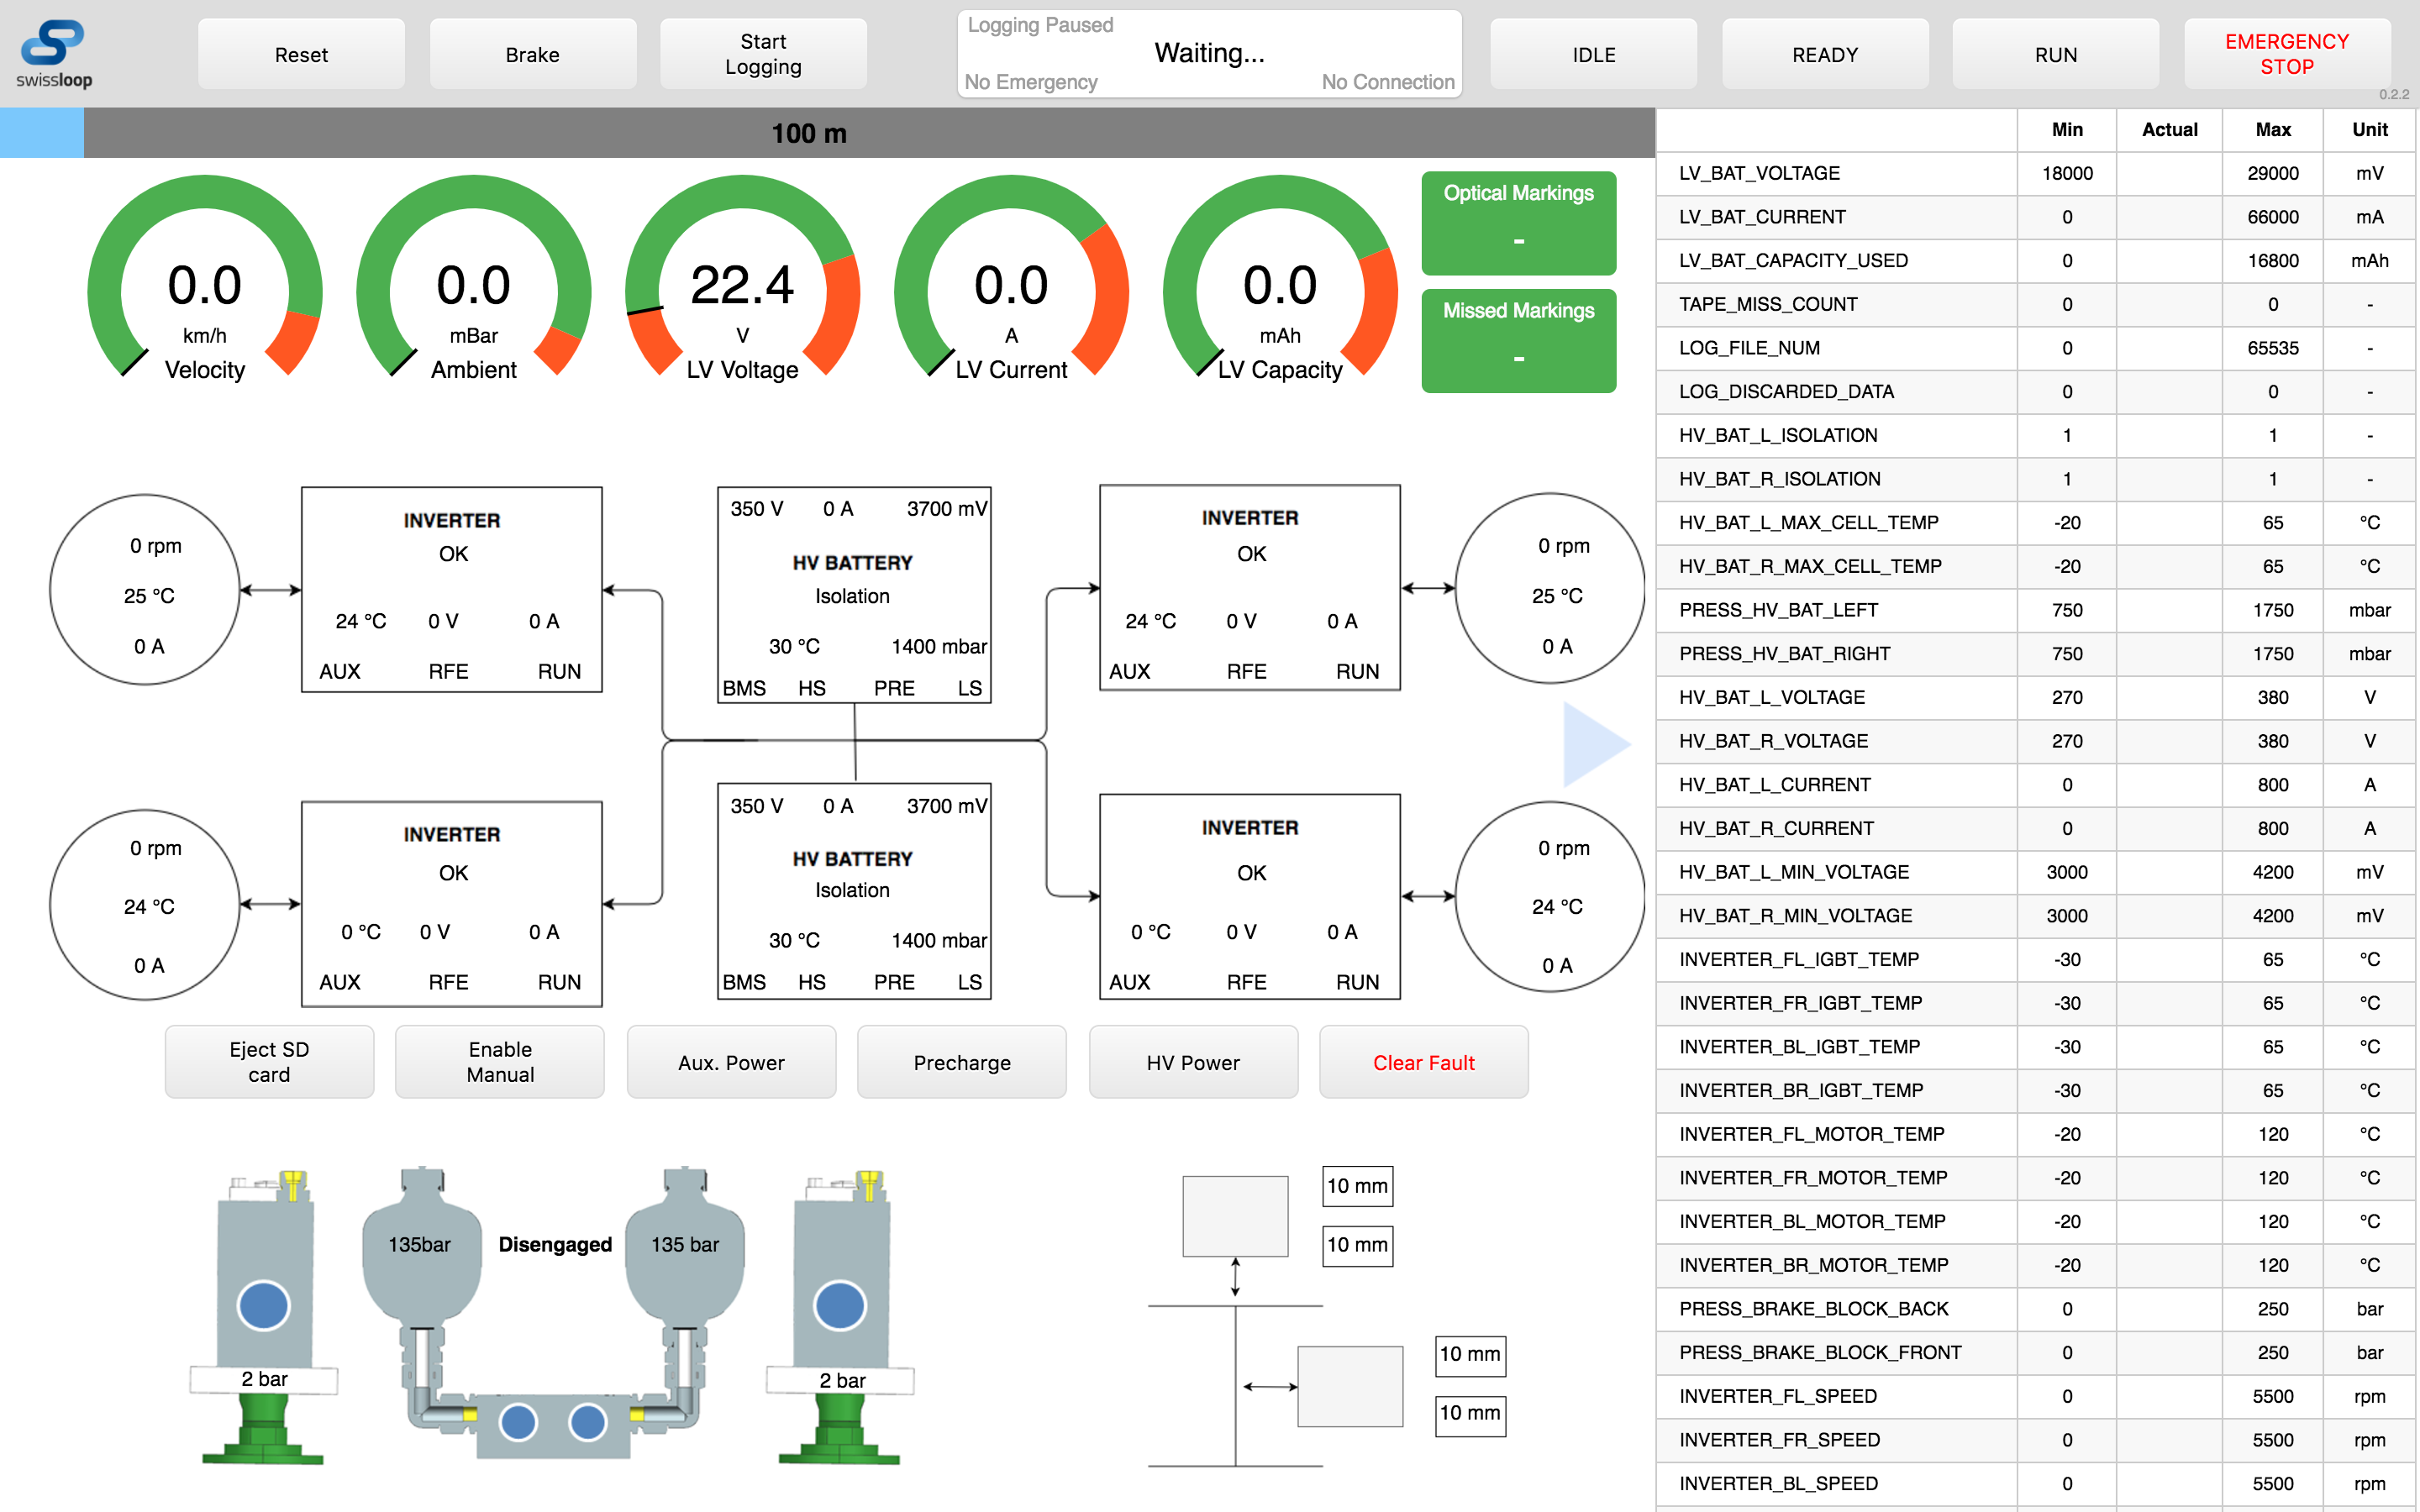
\includegraphics[width=1.0\textwidth]{./figures/Screen_Shot_Control_Panel.png}
  \caption{Screen shot of the control panel.}
\end{figure}

\section{Data Logging}

In order to verify the pod's performance and diagnose possible failures, we wanted to be able to log as much data as possible. Therefore, we set a goal of logging all sensor data that comes into the system.

%\todo{Maybe add screenshot of plotting software?}

\section{Control and State Machine}

Overall, the pod is controlled by a finite state machine (FSM). The FSM must incorporate all critical safety checks and is also used to allow the pod to complete the run autonomously. In order to improve testability, the FSM should have the minimum number of states necessary for the desired functionality. To this end we also decided to minimize the number of automatic state transitions, minimizing the risk of bugs in the implementation.

\section{Correctness and Testability}

The highest priority for this system was to ensure correctness and safety. Therefore it was important to minimize sources of errors and implement the system with testability in mind. Tests include unit tests for individual control sequences and algorithms, as well as functional tests.

\section{Platform}

The hardware platform used for this project is a combination of a custom designed PCB and a Texas Instruments Launchpad (LAUNCHXL-F28379D)\cite{launchpad} featuring the TMS320F28379D micro-controller\cite{mcu}. The Launchpad provides a sold basis which includes all the components necessary to run the micro-controller. It then plugs into the custom PCB which accommodates all the necessary external components and incorporates connectors for all sensors and actuators.

\begin{figure}[H]
  \centering 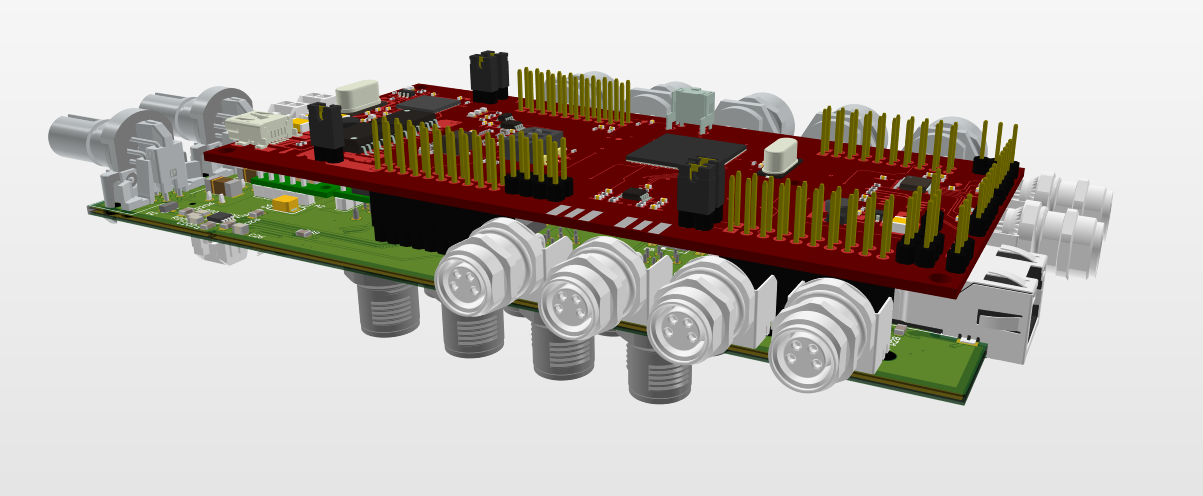
\includegraphics[width=1.0\textwidth]{./figures/pcb.png}
  \caption{Custom PCB with Texas Instruments Launchpad.}
\end{figure}

\subsection{Micro-controller}

The Texas Instruments TMS320F28379D was chosen as it provides high performance in terms of processing with two C28x CPU cores running at 200 MHz and two Control Law Accelerators (CLA). In addition, it incorporates a wide range of versatile peripherals covering most types of interfaces used in the system. Furthermore, this processor is a dual-core version of the single core TMS320F28377S which proved to work very well in Escher.

Texas Instruments also provides a good Runtime Support Library (RTS) for C, as well as header files and support functions as part of ControlSUITE\cite{controlsuite} making it easier to access device registers.

\subsection{Ethernet Controller}

To establish a network connection on the test track an Ethernet connection was required. Since the micro-controller is not equipped with an Ethernet interface it needed to be included externally.

After considering several options we decided on the WIZnet W5500 Ethernet Controller. Beyond providing Ethernet support it also incorporates hardware implementations of ICMP, ARP, IPv4, TCP, UDP and other protocols. This is advantageous as it offloads the computation necessary to run the network stack from the main processor, providing better performance. Furthermore, the chip is widely used and therefore has good community support.

The micro-controller communicates with the Ethernet Controller over SPI but the W5500 also provides an interrupt line which can be configured to provide interrupts on events such as incoming packages.

\subsection{SD-Card}

In order to log telemetry data a form of non-volatile memory was needed. The data must be easily accessible and quickly retrievable. The obvious and most suitable choice is an SD-card, as it can be integrated into the SPI bus and provides large amounts of storage. At the same time it can be easily plugged into a laptop in order to retrieve the data in the field.

\subsection{External Analog-To-Digital Converter (ADC)}

The pressure sensors on the pod produce analog signals that need to be converted. Additionally, the pod incorporates a set of low-voltage batteries and it is necessary to monitor their voltage and discharge current. Although the micro-controller features a built-in 12-bit ADC which could accomplish this task, we wanted to achieve higher precision using an external 24-bit ADC (ADS124S08). Communication with the ADC also runs over an SPI bus. However, the external ADC uses a different SPI mode than the Ethernet Controller and SD-card. Thus a separate SPI bus is required.

\subsection{RS485 Bus}

An objective in the design of this system, was to use as many digital sensors as possible. This was possible for both types of laser distance sensors used on the pod. Both support the RS485 serial bus. Using an appropriate RS485 transceiver, the Serial Communication Interface (SCI) of the micro-controller can be utilized almost natively to communicate with multiple sensors on a single RS485 bus. Unfortunately the two types of sensors use different bus settings and thus it was simpler to separate them into two buses with two sensors each.

RS485 utilizes differential signalling to transmit words asynchronously in the same format as the more widely used RS232 protocol. Since RS485 uses a single differential signal, it is only possible for one device to transmit at a time.

Using the RS485 bus standard means less analog signals that are more prone to interference. Furthermore, it also allows for higher precision, as there are no precision losses during to conversions.

\subsection{CAN Bus}

The motor-controllers (inverters) used on the pod are designed for automotive applications, while the Battery Management Systems (BMS) are designed for aerospace applications. Both systems are designed to use the CAN bus for control and telemetry. The micro-controller incorporates a CAN bus and transceiver on the Launchpad making communication with these devices possible without any additional hardware.

The main advantages of the CAN bus in this application are built-in bus arbitration and automatic retransmission. This allows devices on the CAN bus to transmit telemetry data asynchronously without the possibility of data loss.

%%% Local Variables: 
%%% mode: latex
%%% TeX-master: "../report_template"
%%% End: 

%%%%%%%%%%%%%%%%%%%%%%%%%%%%%%%%%%%%%%%%%%%%%%%%%%%%%%%%%%%%%%%%%%%%%%%
%%%%%%%%%%%%%%%%%%%%%%%%%%%%%%%%%%%%%%%%%%%%%%%%%%%%%%%%%%%%%%%%%%%%%%%
%%%%%                                                                 %
%%%%%     <file_name>.tex                                             %
%%%%%                                                                 %
%%%%% Author:      <author>                                           %
%%%%% Created:     <date>                                             %
%%%%% Description: <description>                                      %
%%%%%                                                                 %
%%%%%%%%%%%%%%%%%%%%%%%%%%%%%%%%%%%%%%%%%%%%%%%%%%%%%%%%%%%%%%%%%%%%%%%
%%%%%%%%%%%%%%%%%%%%%%%%%%%%%%%%%%%%%%%%%%%%%%%%%%%%%%%%%%%%%%%%%%%%%%%

\chapter{Control System Implementation}

The software for the micro-controller was implemented using the C Programming Language. I considered using a real-time operating system but decided that in this case it would be simpler to not to do so. The software runs a main loop and all modules are fundamentally asynchronous. In testing it was possible to show that this yielded very good performance.

Another major design decision is to use only static memory allocation. Although at times this can be limiting and is less space efficient than dynamic memory allocation, it also leads to higher performance. More importantly, this approach guarantees that there are no memory leaks, which can otherwise become fatal bugs that may be difficult to diagnose.

\section{Structure}

Each CPU core runs independently from the other, except during system initialisation. Since some peripherals need to be initialised in the correct sequence and the main loop should not be entered until the entire system is initialised, inter-processor communication (IPC) flags are used to synchronise both cores during start-up.

Each core has dedicated FLASH memory, as well as dedicated RAM regions. Additional shared RAM can be read by both CPUs but only written to by one CPU per block. At boot CPU1 configures the global shared RAM regions according to the applications needs and then sends a command to the boot loader on CPU2 using IPC registers to start the program for CPU2.

\begin{figure}[H]
    \centering 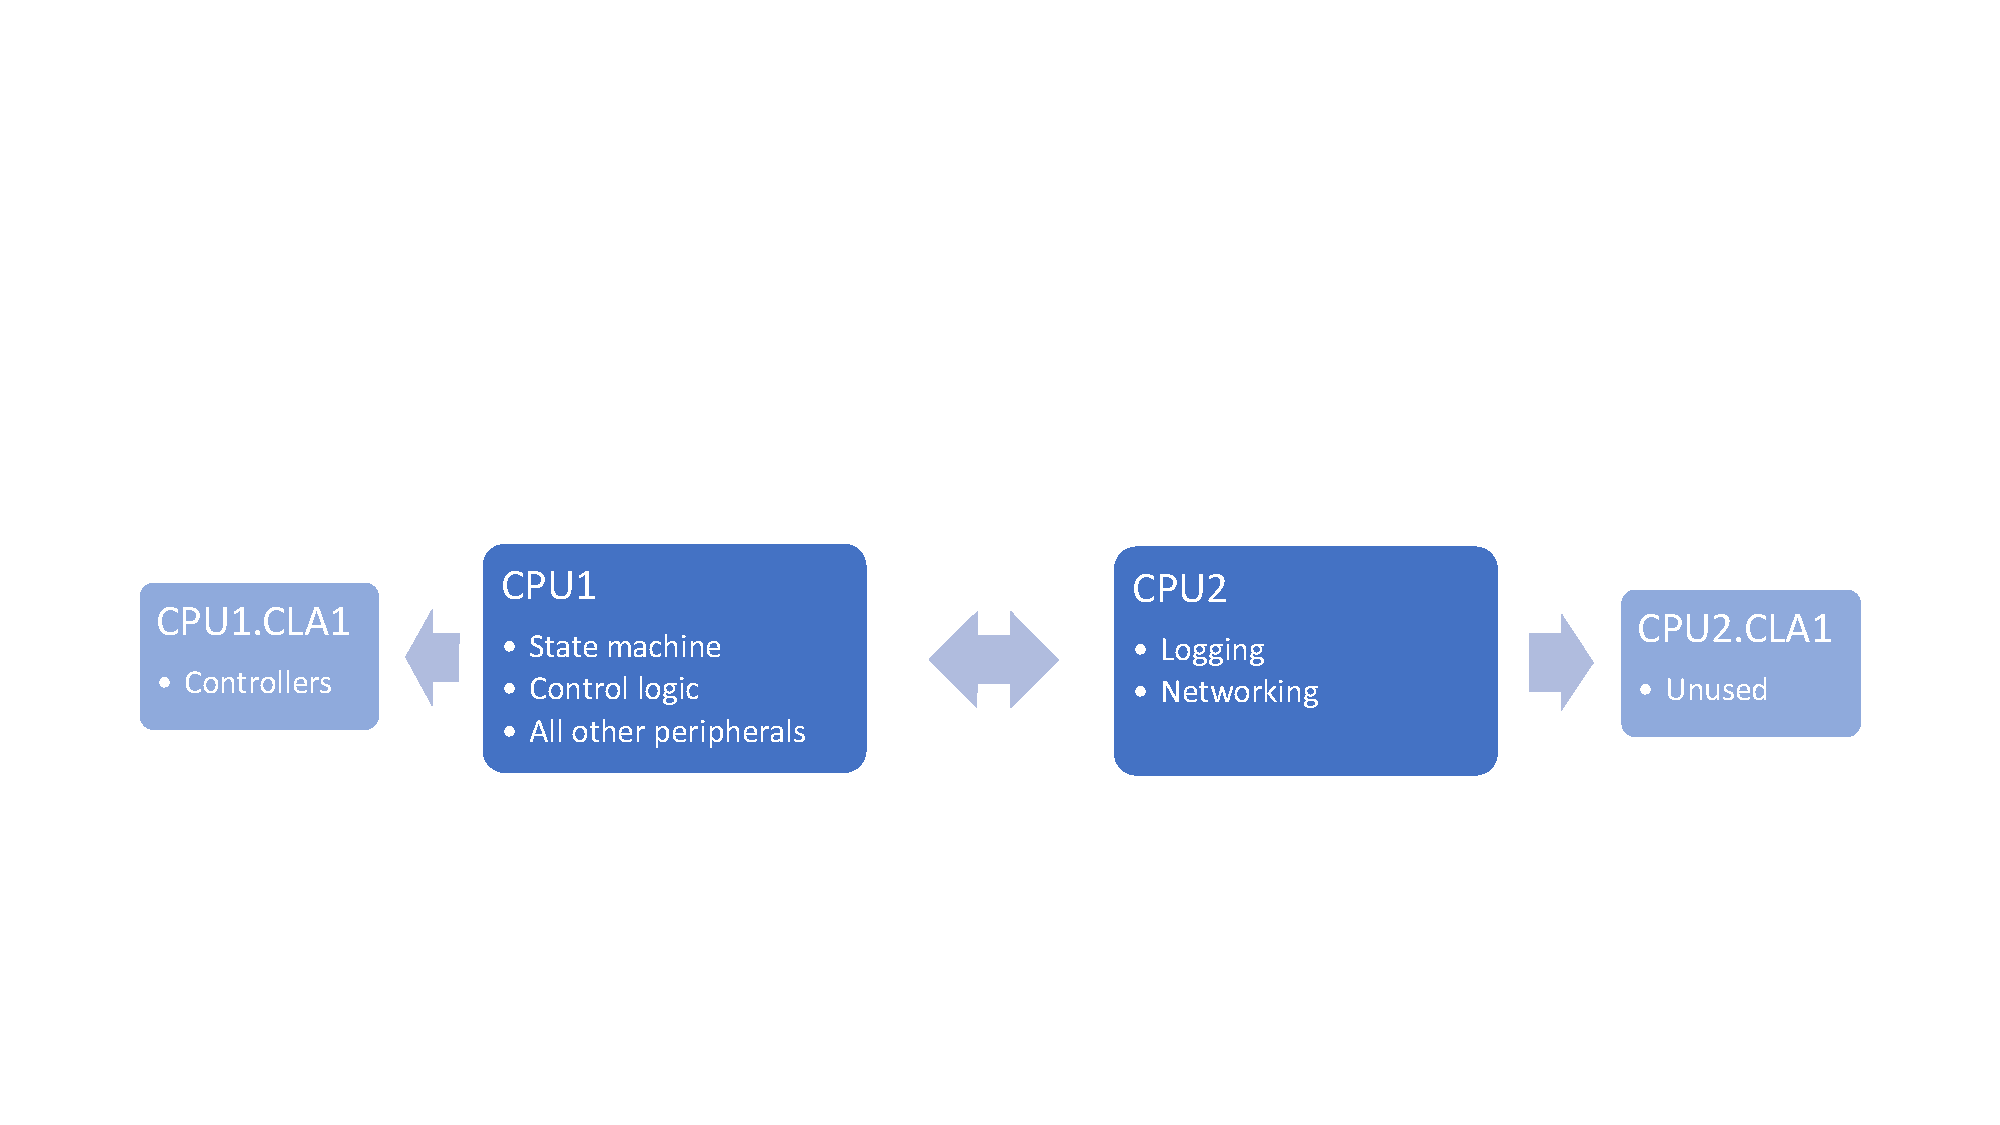
\includegraphics[width=1.0\textwidth]{./figures/system_structure.pdf}
    \caption{Division of tasks between processors and co-processors.}
    \label{fig:system_structure}
\end{figure}

Figure~\ref{fig:system_structure} shows the division of tasks between the two CPU cores and one of the Control Law Accelerator (CLA) co-processors. CPU runs most drivers and handles the control logic and state machine. All sensor data is processed on this core and all control decisions are made on it as well. This consolidates the data processing and control logic in one program with out the need for concurrency control that could be subject to hard to find bugs.

CPU2 is dedicated to Logging and Networking. The main constraint for this is that the FAT file system is computationally heavy and as will be discussed in section~\ref{logging} is hard to implement asynchronously. In order to reduce the performance impact, logging was separated onto the second core. However, since the Ethernet controller uses the same SPI bus as the SD-card and only one CPU core can be the master of each peripheral (in this case one of the SPI interfaces), networking also needs to be handled on the second core.

The traction and yaw controllers must run regularly in precise intervals and therefore somewhat contradict the asynchronous nature of the remaining system. Furthermore, as they were developed by other people who did not necessarily have detailed knowledge of the system, it made sense to provide an isolated environment for the execution of the controllers.

The CLA co-processor runs at the same frequency as the associated CPU core but executes code independently. It is assigned areas of the associated CPU's dedicated RAM for program and data space. As the CLA co-processor is designed to run controllers, it can be assigned up to eight function pointers, which represent tasks. These tasks can be triggered from peripherals but also from software running on the CPU. Once a task is triggered, it runs to completion. Although the instruction set for the CLA is separate and significantly more limited, these other features make the CLA perfectly suited for the task.

\subsection{Module life-cycle}

All modules and drivers follow a similar structure. This structure mainly consists of three functions that are called at different times during the module life-cycle as illustrates in Figure~\ref{fig:module_lifecycle}: \mintinline{c}{init()}, \mintinline{c}{configure()} and \mintinline{c}{update()}.

\begin{figure}[H]
    \centering 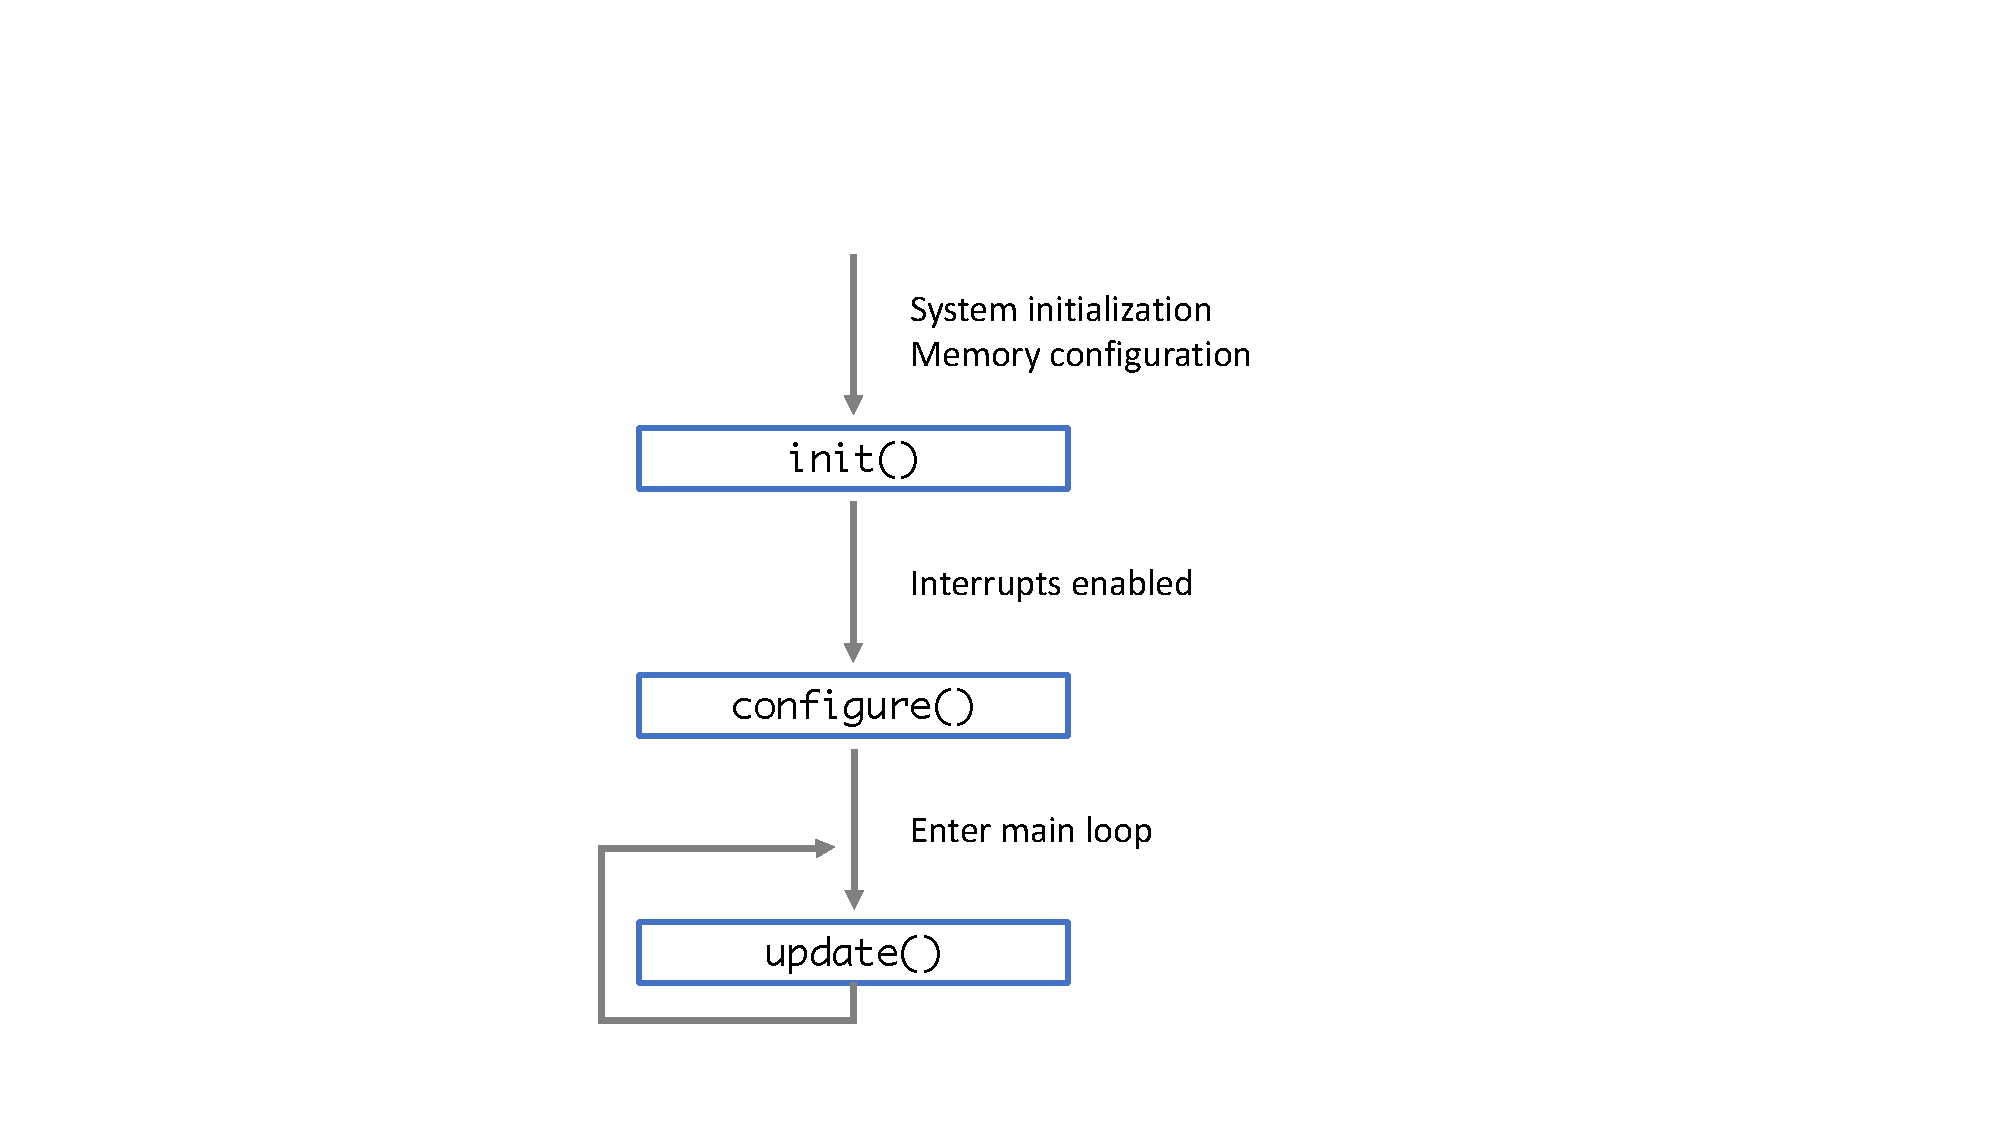
\includegraphics[width=0.5\textwidth]{./figures/module_lifecycle.pdf}
    \caption{Life-cycle of each module in the system.}
    \label{fig:module_lifecycle}
\end{figure}

Immediately after system initialization and memory configuration is complete, \mintinline{c}{init()} is called to allow modules to perform initialisation routines, configure peripherals and enable required interrupts. However, interrupts remain globally disabled for the duration of these function's execution.

Some drivers require further initialisation after interrupts have been enabled. Mostly this involves the configuration of an external device such as the Ethernet Controller, SD-card and laser distance sensors. For these initialisation sequences require fully functional communication and therefore interrupts. This is the purpose of the \mintinline{c}{configure()} functions.

After start-up is complete the processor enters the main loop. At each iteration of the loop the \mintinline{c}{update()} function of each module is called. If the module does not need to perform any computation at that time it immediately returns. Several modules use internal finite state machines in order to allow for asynchronous execution.

\subsection{Data-flow}

\begin{figure}[H]
    \centering 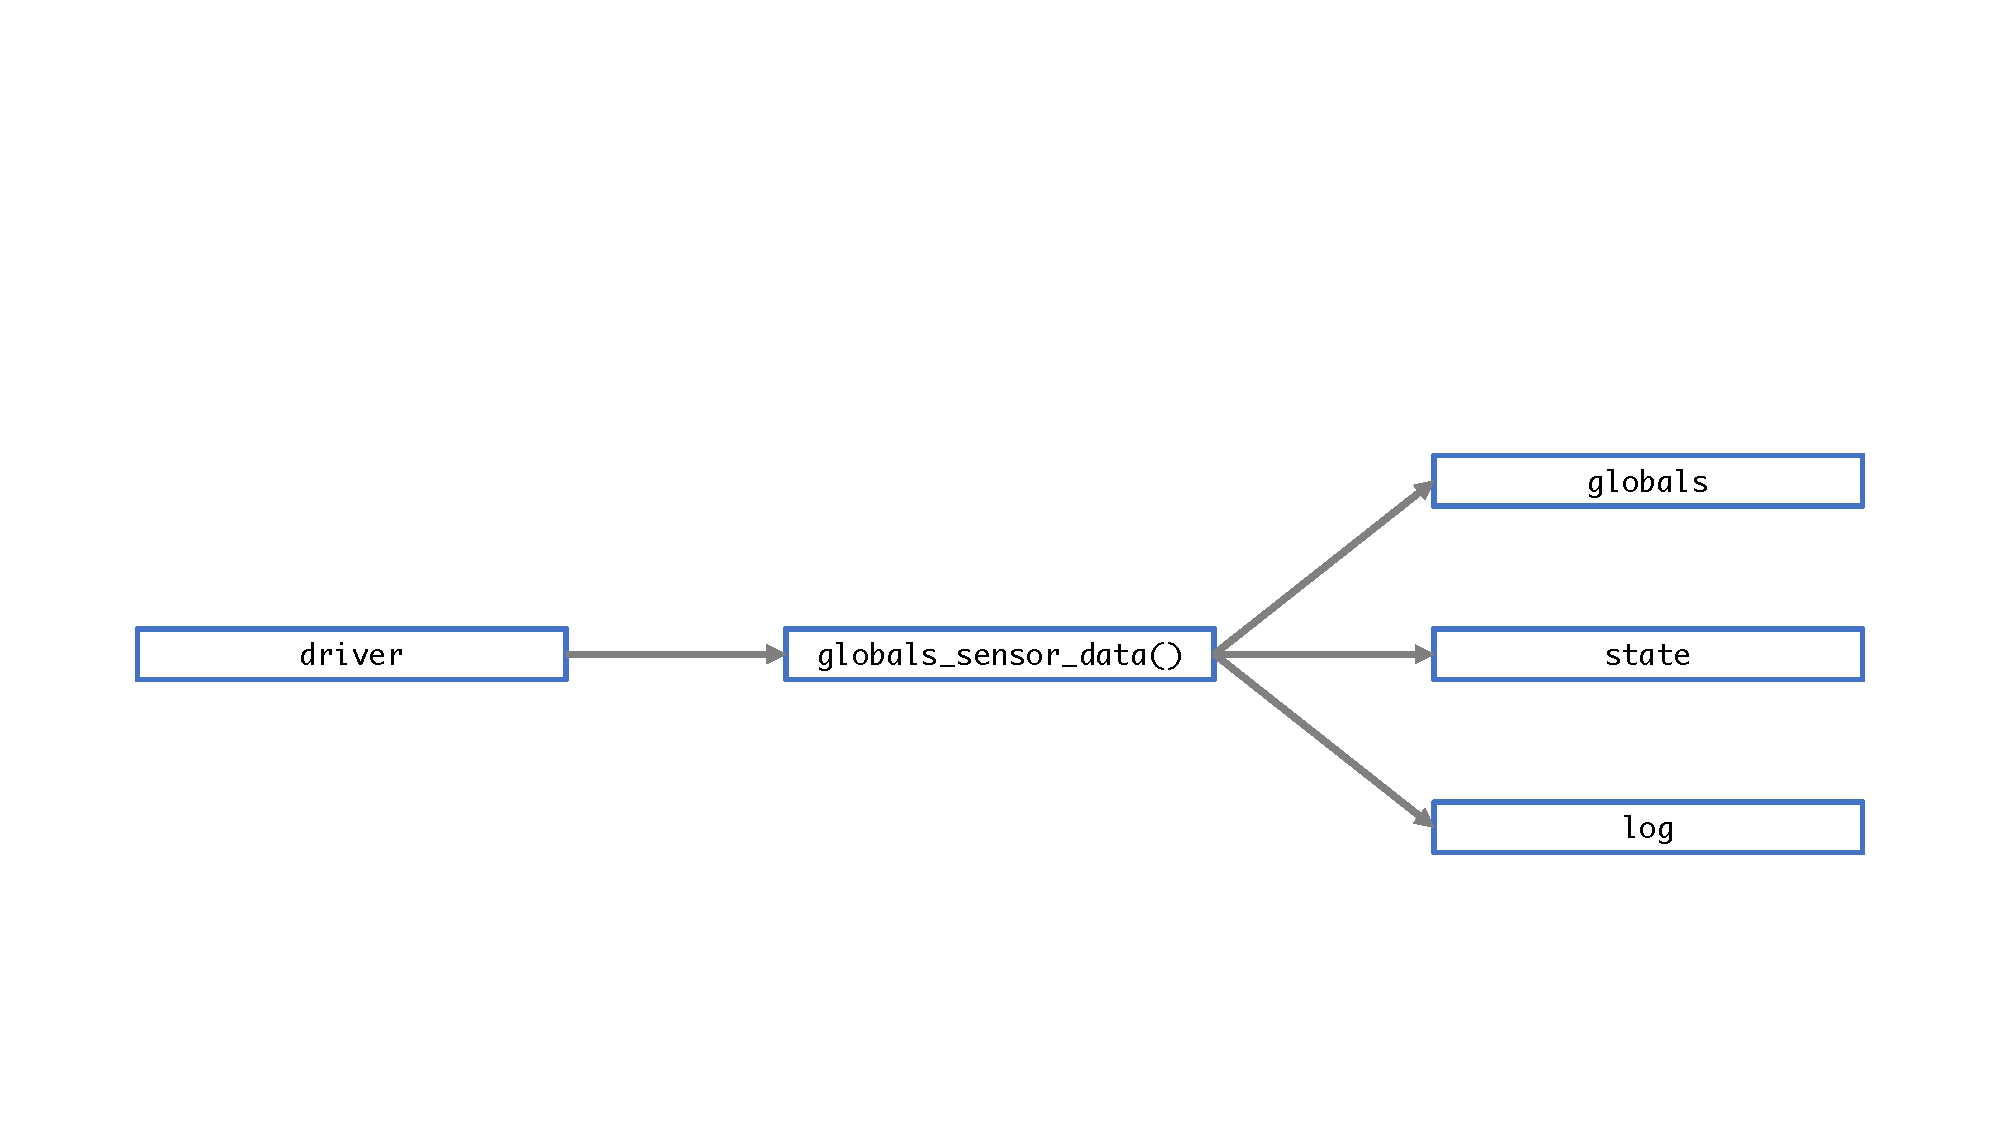
\includegraphics[width=1.0\textwidth]{./figures/dataflow.pdf}
    \caption{Flow of sensor data and derived data.}
    \label{fig:dataflow}
\end{figure}

All data processing is centralised using the \mintinline{c}{globals_sensor_data()} function. The concept is to simplify how data is distributed throughout the program. Drivers call \mintinline{c}{globals_sensor_data()} whenever a new data point is gathered from a sensor. Derived data such as velocity or location is also collected through this function. In this way the data flow is abstracted from the driver layer improving modularisation, maintainability and flexibility.

Once a data point has been collected by a call to \mintinline{c}{globals_sensor_data()}, the data can be stored to a global structure for use by other modules and used to to update the global finite state machine. Additionally, all data points are logged as will be described in Section~\ref{logging}.

\section{Networking}

The network protocol needs to be resistant to packet loss and unstable network connections, while still providing a steady stream of data. Unlike the event-based logging system (Section~\ref{logging}) telemetry data transmitted over the network can be relatively infrequent and there is no data that must be delivered at a higher rate than other data. Therefore I implemented the protocol using UDP packets. The structure listed in Appendix~\ref{telemetry_frame} holds all the data that needs to be transmitted. It fits into a single UDP packet without segmentation. This makes it very efficient to transmit telemetry and resistant to occasional packet loss as only one packet is needed to observe the pod's state.

For controlling the pod remotely from the control panel the protocol follows an analogous scheme using a control frame consisting of the following structure.

\begin{minted}{c}
struct ctrl_frame {
    uint16_t set_state;     // 0: D.C. / ..: the state
    uint16_t aux_power;     // 0: D.C. / 1: OFF / 2: ON
    uint16_t precharge;     // 0: D.C. / 1: OFF / 2: ON
    uint16_t battery;       // 0: D.C. / 1: OFF / 2: ON
    uint16_t brakes;        // 0: D.C. / 1: DISENGAGE / 2: ENGAGE
    uint16_t low_speed;     // 0: D.C. / 1: BACK / 2: STOP / 3: FWD
    uint16_t clear_fault;   // 0: D.C. / 1: CLEAR
    uint16_t reset_run;     // 0: D.C. / 1: RESET
    uint16_t bms_power;     // 0: D.C. / 1: OFF / 2: ON
    uint16_t eject_sd_card; // 0: D.C. / 1: EJECT
};
\end{minted}

Both the telemetry frame and control frame must be sent (and received) regularly in order for the pod and the control panel to check connectivity and enter a safe state should it fail. Therefore the fields in the control frame are usually zero and a non-zero value indicates a control command.

Although the networking drive primarily executes on CPU2, a small portion also executes on CPU1. This is necessary, since all telemetry data originates from CPU1. Rather than placing data in global structures unnecessarily, the telemetry frame is simply assembled on CPU1 and then read by the DMA controller on CPU2. Similarly, CPU2 receives incoming control packets and CPU1 decodes them and executes any control commands. This process is illustrated by Figure~\ref{fig:networking_structure}.

\begin{figure}[H]
    \centering 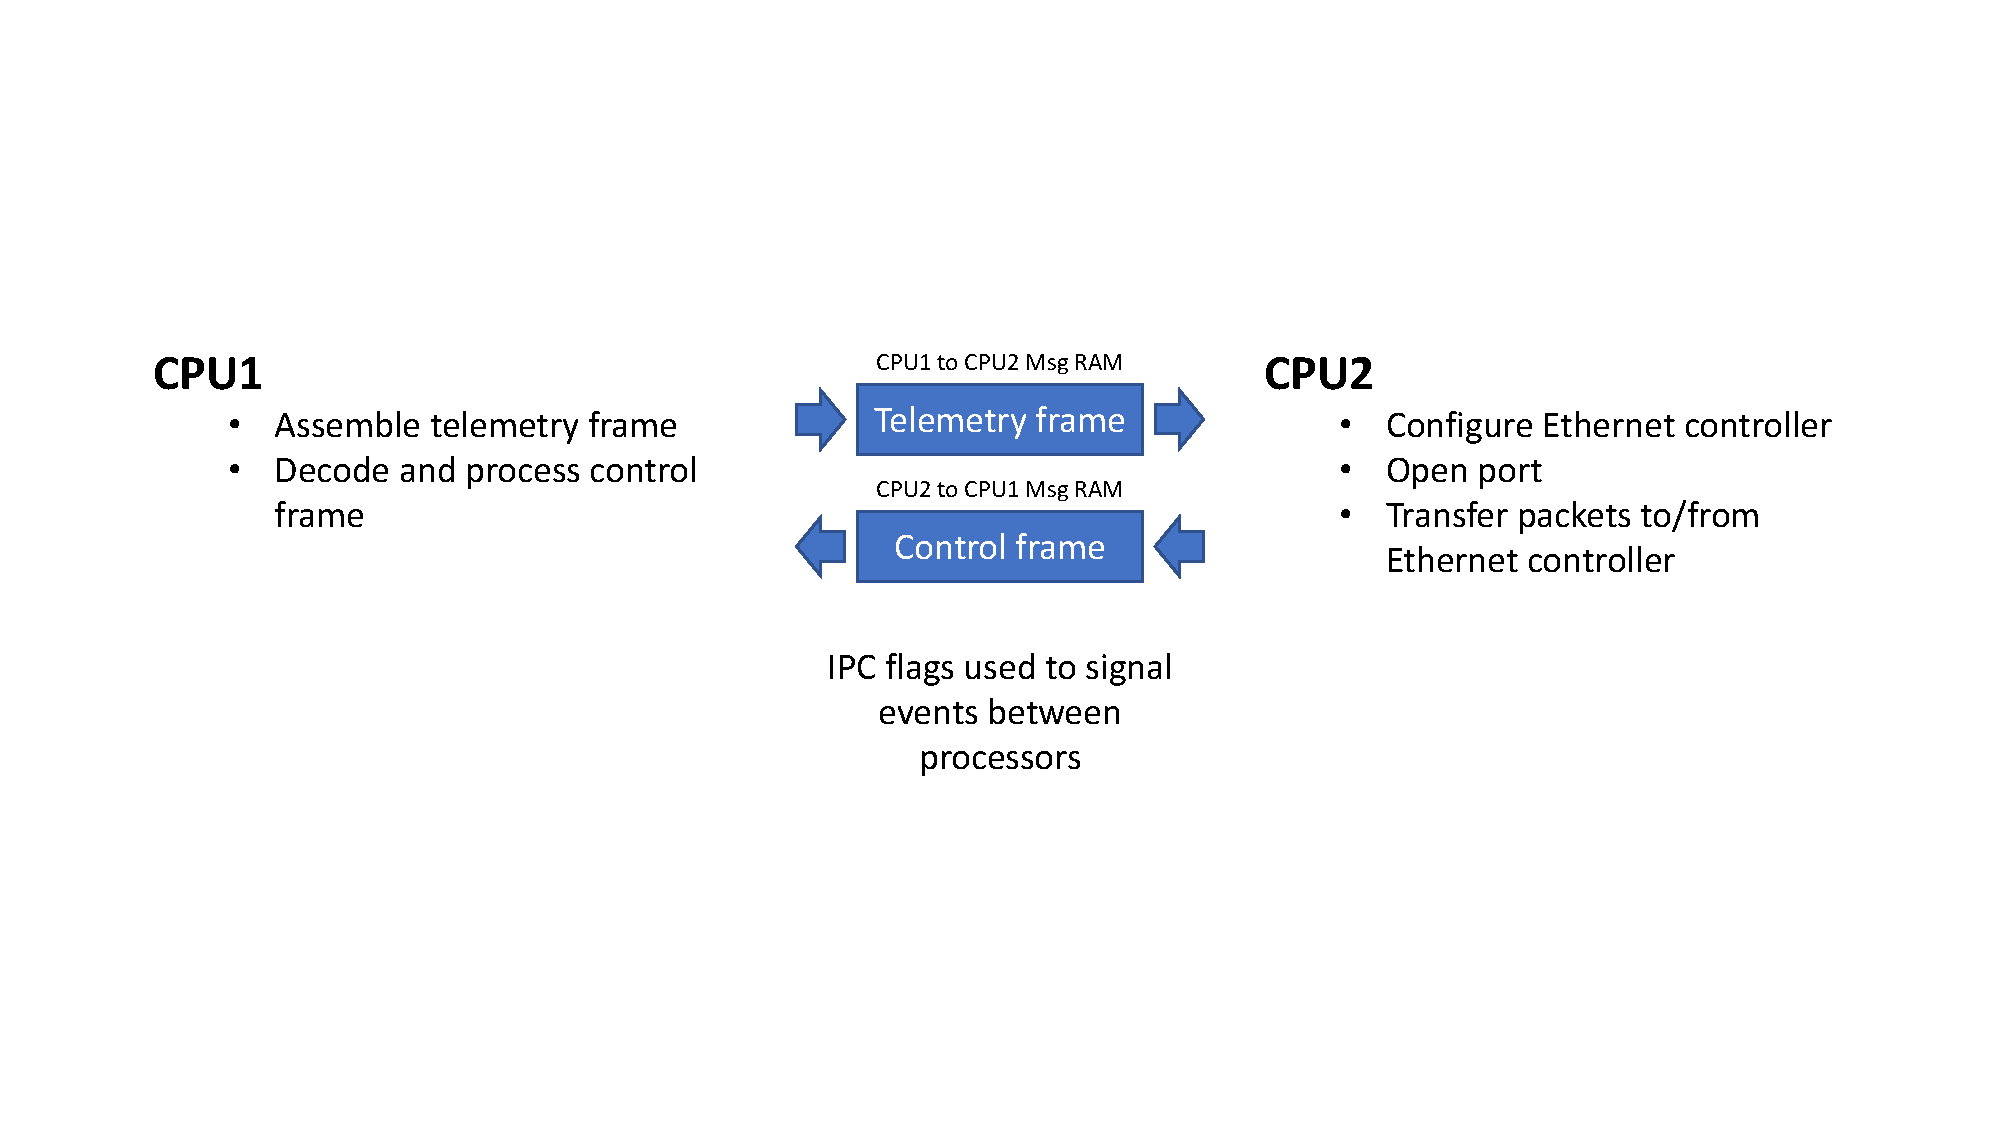
\includegraphics[width=1.0\textwidth]{./figures/networking_structure.pdf}
    \caption{Structure of networking driver.}
    \label{fig:networking_structure}
\end{figure}

The telemetry and control frames are written to Message RAM, which is a shared memory area specifically designed for this kind of usage. It consists of two 1K regions, one writeable only by CPU1 and one only writeable by CPU2. The telemetry frame only consists of 76 16-bit words and therefore easily fits into the Message RAM. The micro-controllers Interprocessor Communication (IPC) module further provides flag registers. The networking driver uses IPC flags to notify the other CPU of the following events:

\begin{itemize}
    \item CPU1 $\rightarrow$ CPU2: Telemetry frame assembled and ready for transmission.
    \item CPU2 $\rightarrow$ CPU1: Telemetry frame has been transmitted and can be overwritten.
    \item CPU2 $\rightarrow$ CPU1: Control frame received.
    \item CPU1 $\rightarrow$ CPU2: Control frame has been processed and can be overwritten.
\end{itemize}

To achieve the highest possible performance all SPI communication with the Ethernet controller is implemented using the micro-controller's DMA controller. Since the SPI interface can be used with a 16-level FIFO extension, the DMA controller can operate in Burst mode. This means that the data is transferred in bursts of 16 words until the transfer has completed. The next bust is triggered by the FIFO interrupt which can be configured to assert at a specific level. For this implementation it is configured to trigger when the FIFO is empty but depending on the size of the bursts this can be optimized.

The following listing shows the process of configuring channel one of the DMA controller for transmission of a buffer at \mintinline{c}{src} of length \mintinline{c}{len}. Notice that the burst length must be a divisor of the total buffer size. This is because the DMA controller cannot handle bursts of different lengths.

\begin{minted}{c}
void spia_tx_dma(uint16_t *src, uint16_t len)
{
    uint16_t burst;

    // Calculate largest burst length
    for (burst = 16; len % burst; burst /= 2) ;

    // Reset the TX FIFO
    SpiaRegs.SPIFFTX.bit.TXFIFO = 0;

    // Configure DMACH1 for SPIA TX
    DMACH1AddrConfig(&SpiaRegs.SPITXBUF, src);
    DMACH1BurstConfig(burst - 1, 1, 0);             // Burst size, src step, dest step
    DMACH1TransferConfig((len / burst) - 1, 1, 0);  // Number of transfers, src step, dest step
    DMACH1ModeConfig(DMA_SPIATX,PERINT_ENABLE,ONESHOT_DISABLE,CONT_DISABLE,
                     SYNC_DISABLE,SYNC_SRC,OVRFLOW_DISABLE,SIXTEEN_BIT,
                     CHINT_END,CHINT_ENABLE);

    // Set the TX FIFO interrupt level
    SpiaRegs.SPIFFTX.bit.TXFFIL = 0;

    // Start the DMA transfer
    _spia_tx_dma_done = 0;
    StartDMACH1();

    // Release the TX FIFO from reset
    SpiaRegs.SPIFFTX.bit.TXFIFO = 1;

}
\end{minted}

The procedure for configuring the DMA controller to read data from the SPI interface is analogous.

Using the DMA controller means that the SPI interface can operate at it's highest possible data-rate without causing significant CPU usage. The clock rate used for the SPI bus is 12,5 MHz.

\section{Logging} \label{logging}

\subsection{File system}

The largest design decision in designing the logging driver was the file system to use. The main requirement was for the logged data to be quickly and easily retrievable. The most commonly used file system on SD-cards is FAT (FAT32 or exFAT). The advantage of the FAT file system in this case is that it can be read with almost any computer making it particularly easy to retrieve log files. On the other hand, FAT is very inefficient unless the FAT table (which on larger storage devices is very large) can be cached in memory. If the FAT table is not cached, it must be read block by block every time a file is being written and a new block is needed. In embedded applications like this one, it is usually not possible to cache the FAT table.

Instead of using FAT I also considered employing specialized logging file systems such as log\_fs \todo{insert reference} and Yaffs \todo{insert reference}. These sequentially write to the storage medium and do not need to access any other data structures while writing the file. Although this leads to higher performance while writing, it also makes finding and extracting log data much more complex. Furthermore, it is not possible to read the data on a regular computer without specialised software. For this reason, I decided to use the FAT file system and write the log data to CSV files.

Log files are created at system start-up and data is continuously appended until the system shuts down or a manual command is given to close the file and ensure data consistency. The CSV file consists of three columns:

\begin{itemize}
    \item \textbf{timestamp}: The time stamp of the data point measured in milliseconds since system start-up.
    \item \textbf{id}: An integer describing the type of data point or event being logged. IDs are defined by the enumeration listed in Appendix~\ref{log_event}
    \item \textbf{value}: The value being logged.
\end{itemize}

The following listing illustrates the structure of a typical log file:

\begin{verbatim}
timestamp;id;value
4778;41;7
4778;39;348
4778;40;3820
4778;42;24
4778;45;5
4778;43;352
4778;44;3781
4778;46;26
4778;5;0
4778;4;0
4879;38;0
4879;37;0
4879;36;0
4879;1;6
4879;2;4
\end{verbatim}

Although beneficial, implementing a specialised FAT driver would not have been possible within the time-frame of this project. Therefore, I decided to use the FatFs\todo{reference} library. At first I attempted to use the newest version of the library. However, the micro-controller uses 16-bit addressable memory and therefore does not support 8-bit data types. Without rewriting large portions of the library it was not possible for it to run without native 8-bit data types. Luckily Texas Instruments includes an older version of the library with ControlSUITE\todo{reference} that is able to run without 8-bit data types.

The FatFs library provides the file system library but an SD-card driver layer also needed to be implemented to provide the interface to the underlying storage medium through the SPI driver. Unlike all other drivers, the SD-card and FAT drivers are not asynchronous. This is mostly due to how the FatFs library operates. Additionally, the data is organized into 8-bit bytes each contained within a 16-bit word which is the smallest possible data type on the processor. Furthermore, due to this constraint the use of DMA is not practical as data mapping is necessary before data can be written to the SPI interface and after it is read from the SPI interface.

Due to the limitations described above, the entire logging driver is fundamentally synchronous and the SD-card driver is implemented using only the FIFO extension of the SPI interface and without DMA. Given more time, a custom FAT driver could be designed specifically for this processor and incorporate the DMA controller and asynchronous operation. Alternatively, a real-time operation system could be used to partially alleviate the problem using threading. Another crude fix to introduce some asynchronism would be to utilize long jumps to context switch out of the logging driver.

\subsection{Event-based logging}

In the logging system implemented in Escher, logging and telemetry data transmission were coupled. The main disadvantage to this was that all data values were logged at the same frequency and no prioritization was possible. Although most sensors on Escher were sampled at the same rate, this is not the case on Mujinga where some sensors such as the the laser distance sensors are sampled at around 150Hz and others such as the brake pressure sensors are sampled at 10Hz. Thus, in contrast to Escher, Mujinga's logging system is event-based.

Whenever a new data point is acquired or another system event occurs, a string corresponding to a line in the CSV log file is generated and appended to a buffer. The following listing shows the procedure for generating the string:

\begin{minted}{c}
// Buffers used to construct string
// ( 8) timestamp (ms)
// ( 1) ;
// ( 5) id
// ( 1) ;
// (20) value
// ( 3) \r\n\0
static char string[38], temp[21];

// Write timestamp
itoa(micros() / 1000, string);

// Write ';'
strcat(string, ";");

// Write id
itoa(id, temp);
strcat(string, temp);

// Write ';'
strcat(string, ";");

// Write value
itoa(value, temp);
strcat(string, temp);

// Write "\r\n"
strcat(string, "\r\n");
\end{minted}

\subsection{Dual-core structure}

Similar to the networking driver, the logging driver is also divided between both cores since all data that needs to be logged is generated on CPU1 while CPU2 maintains the file system and writes to the log file. Figure~\ref{fig:logging_structure} illustrates the cross-core structure.

\begin{figure}[H]
    \centering 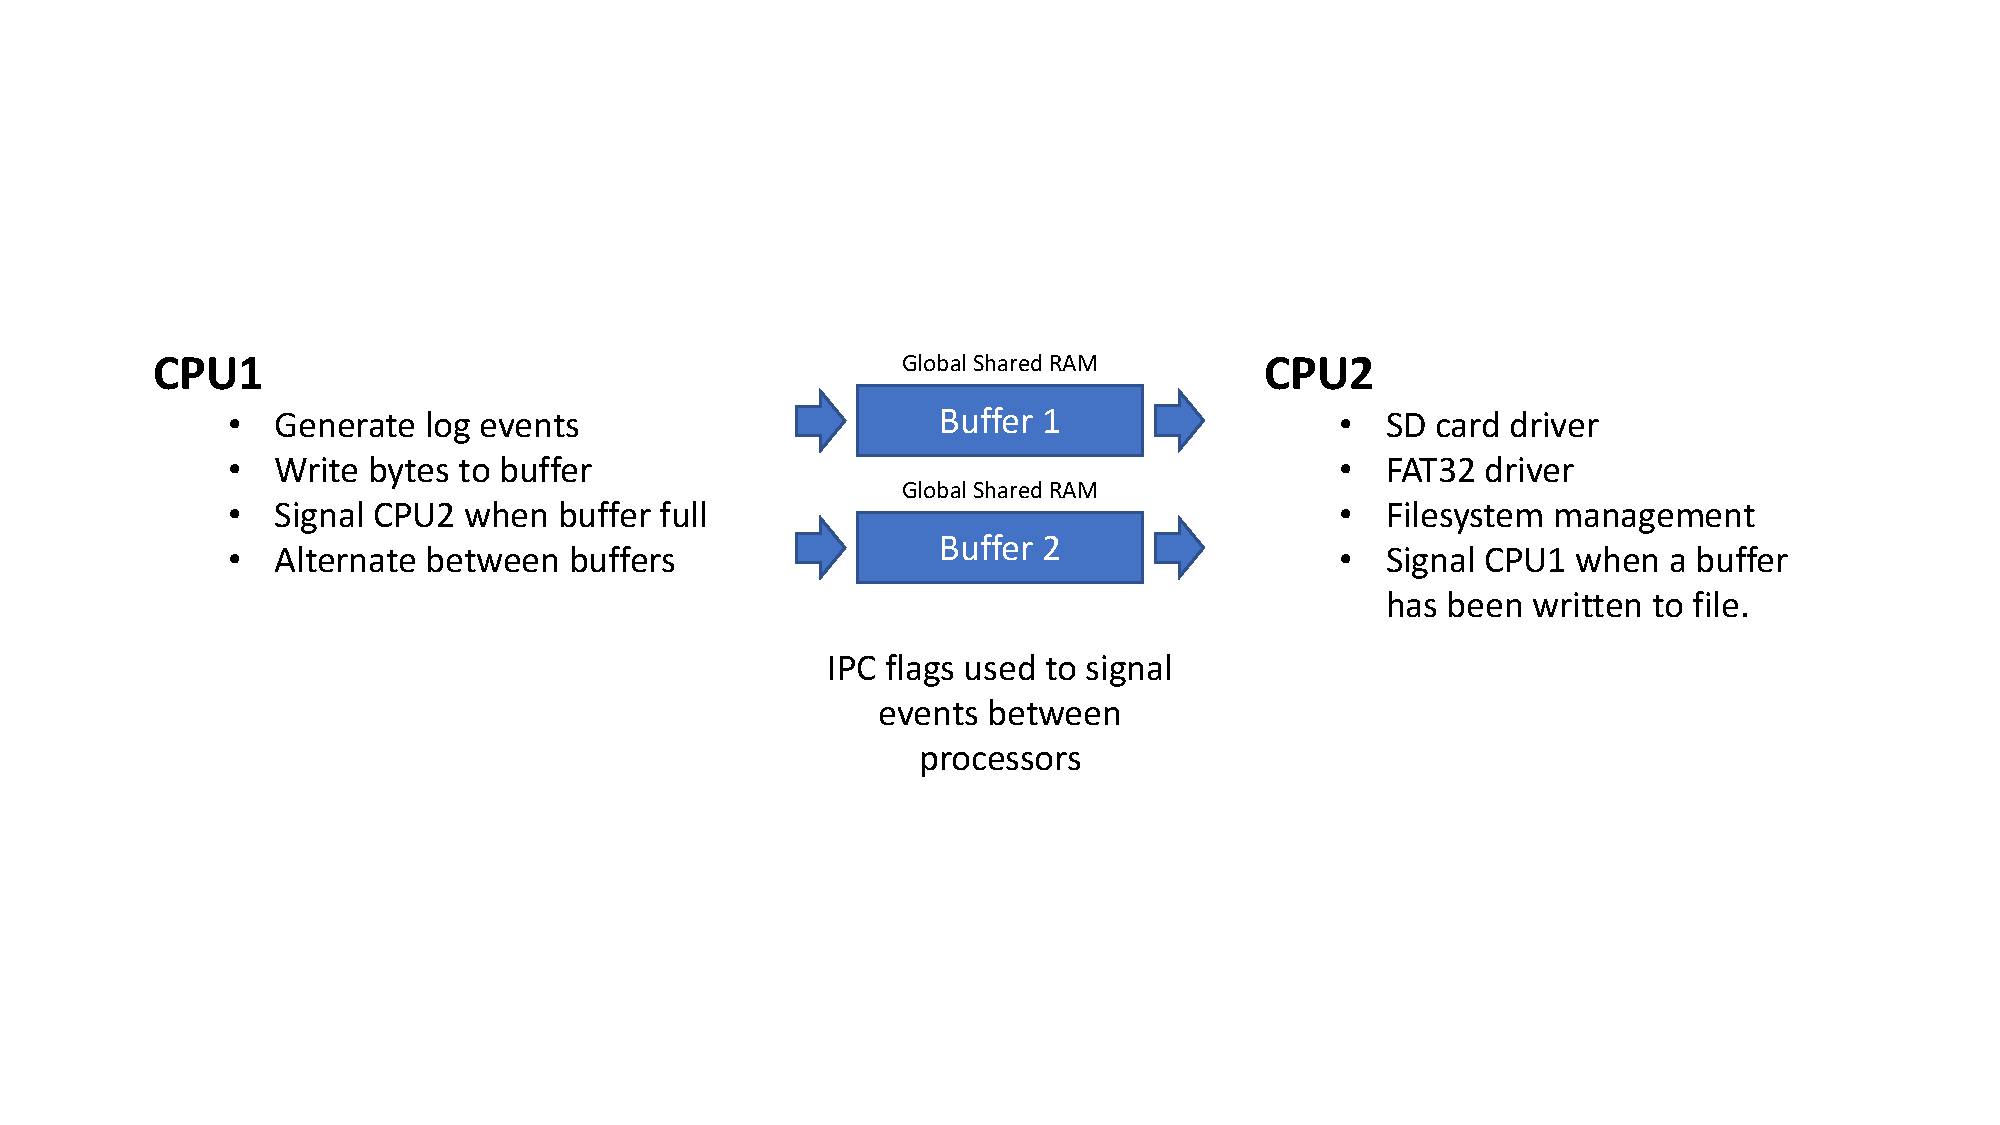
\includegraphics[width=1.0\textwidth]{./figures/logging_structure.pdf}
    \caption{Structure of logging driver.}
    \label{fig:logging_structure}
\end{figure}

Two buffers in shared memory (writeable by CPU1) are used to hold the next segments of the log file as they are generated. Once a buffer is full an IPC flag is used to communicate this to CPU2 and CPU1 continues to write to the other buffer. CPU2 writes the buffer out to the SD-card. Once this is complete it uses an IPC flag to signal to CPU1 that the buffer can be overwritten again and the process repeats.

Usually this kind of functionality would be achieved using a ring-buffer. However, in this particular situation this approach does not work as well for two reasons:

Firstly, for performance reasons relating to the SD-card, performance is best when the file is written in consecutive blocks of 512 byte. Additionally, this reduces the overhead produced by reading the FAT table since every block will only be accessed to once.

Secondly, to optimized the performance of the FatFs library by reducing overheads, the write operation should be invoked infrequently with large chunks of data rather than frequently with smaller chunks of data. When using a ring-buffer a chunk of data may not be consecutively stored in memory leading to at least two invocations of the write operation rather than one.

Given these constraints, an optimally implemented and configured ring-buffer would operate identically to the separate buffers approach explained above. Each buffer consists of 4kB. The trade-off leading to this size is explained in Section~\ref{logging_perf}.

\section{External Analog-To-Digital Converter (ADC)}

Driver implementation and optimization.

\section{RS485 Bus}

General RS485 structure with SCI and transceiver. FIFO usage. RTS solution.

\subsection{OADM}

\subsection{OM70}

\section{CAN Bus}

General CAN structure. CAN driver from TI.

\section{Inverters}

Structure. State machine.

\section{BMS}

Structure. Event-based data.

\section{Navigation algorithm}

\section{State Diagram}

\section{Control Law Accelerator (CLA)}

\begin{figure}[H]
    \centering 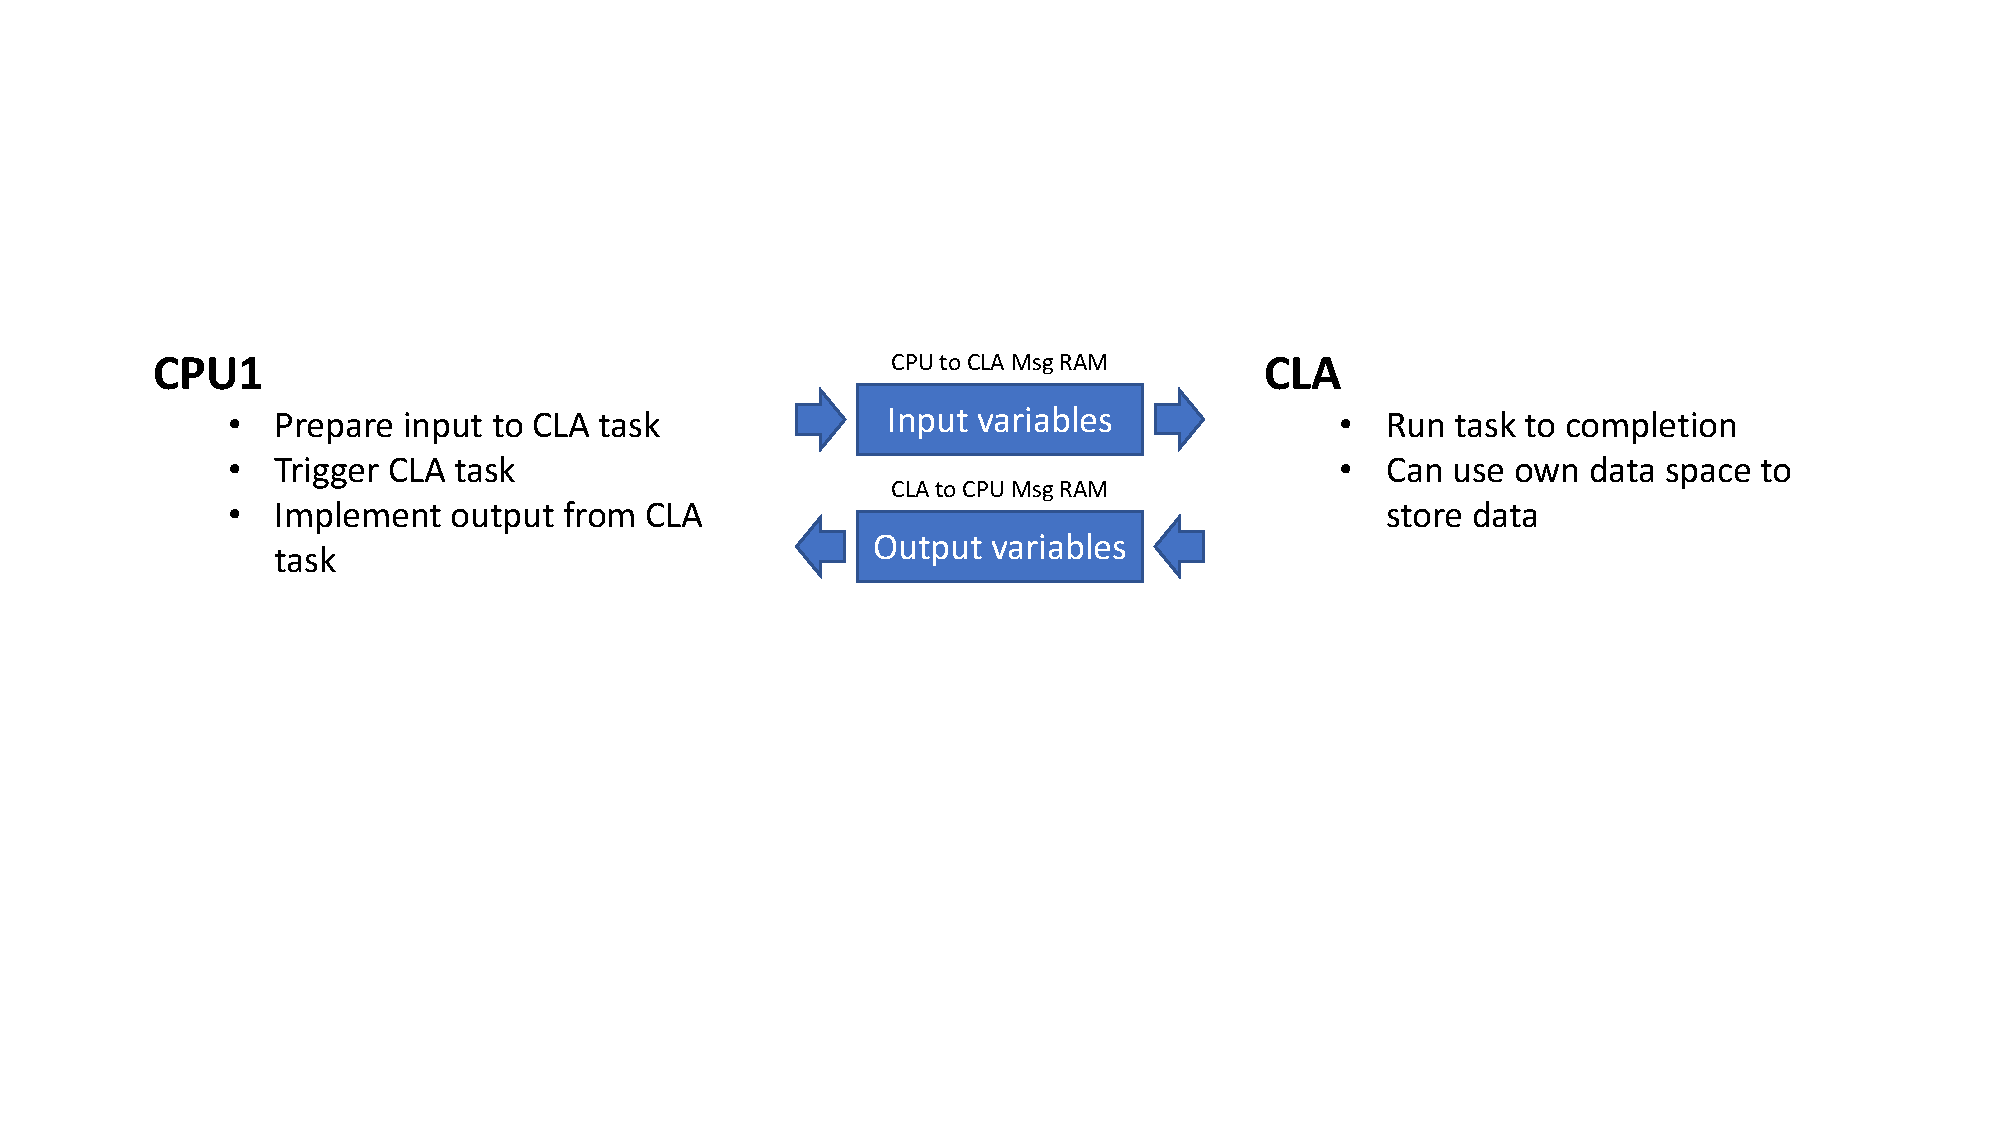
\includegraphics[width=1.0\textwidth]{./figures/CLA_communication.pdf}
    \caption{Communication of inputs ant outputs for CLA tasks.}
    \label{fig:CLA_communication}
\end{figure}

\section{Debugging}

Smaller footprint printf library. Cross-core communication for printing

\section{Unit Testing}

%%%%%%%%%%%%%%%%%%%%%%%%%%%%%%%%%%%%%%%%%%%%%%%%%%%%%%%%%%%%%%%%%%%%%%%
%%%%%%%%%%%%%%%%%%%%%%%%%%%%%%%%%%%%%%%%%%%%%%%%%%%%%%%%%%%%%%%%%%%%%%%
%%%%%                                                                 %
%%%%%     <file_name>.tex                                             %
%%%%%                                                                 %
%%%%% Author:      <author>                                           %
%%%%% Created:     <date>                                             %
%%%%% Description: <description>                                      %
%%%%%                                                                 %
%%%%%%%%%%%%%%%%%%%%%%%%%%%%%%%%%%%%%%%%%%%%%%%%%%%%%%%%%%%%%%%%%%%%%%%
%%%%%%%%%%%%%%%%%%%%%%%%%%%%%%%%%%%%%%%%%%%%%%%%%%%%%%%%%%%%%%%%%%%%%%%


\chapter{Experimental Results}

\section{Performance Evaluation}

\subsection{Logging and SD-card driver} \label{logging_perf}

Experimental evaluation of the SD-card driver by visualising write operations using an oscilloscope attached to the SPI bus revealed an important trade-off that greatly impacts the performance of the logging driver. Although many overheads are introduced by the FAT file system, the SD card also introduces an overhead during read and write operations. As write operations are more relevant in this particular application the following will examine only write operations.

Figure~\ref{fig:sd_card_write} illustrates the initial steps of writing to an SD-card. First a write command is issued. This is then followed by one or more data packets consisting of a data token, 1-2048 bytes of data and two CRC bytes. Between the cursors in Figure~\ref{fig:sd_card_write} one data packet is transmitted. Once all the data packets have been transmitted, a write termination command is transmitted. This last command is omitted if a single block write operation is used.

\begin{figure}[H]
    \centering \includegraphics[width=1.0\textwidth]{./figures/"SPI SD WRITE".PNG}
    \caption{Write command and data packet on SPI bus with SD card.}
    \label{fig:sd_card_write}
\end{figure}

Between each data packet and after the full sequence of commands and packets, the SD card enters a busy state where it is processing the written data. As Figure~\ref{fig:sd_card_write_wait} shows, the busy time after the full sequence (or rather after the write termination command) is particularly long in relation to the transmission time of a single data packet.

\begin{figure}[H]
    \centering \includegraphics[width=1.0\textwidth]{./figures/"SPI SD WRITE1".PNG}
    \caption{Wait time after writing data packet to SD card.}
    \label{fig:sd_card_write_wait}
\end{figure}

Further testing revealed that, while the busy time between data packets is very small, the busy time is almost completely dominated by the busy time at the end of a write operation. This is further verified by another test where chunks of different sizes are repeatedly written to a file in the FAT file system and the data rate observed. Table~\ref{tab:write_speed} shows the results of this test. As can be seen from Figure~\ref{fig:write_speed} the write speed behaves almost linearly compared to the chunk size.

\begin{table}[htbp]
    \caption{Write speeds for chunks of different sizes.}
    \label{tab:write_speed}
    \centering\begin{tabular}{@{}lcr@{}} \toprule
    \textbf{Chunk size} & \textbf{Average data-rate} \\ \midrule
        256 bytes & 21 kB/s \\
        512 bytes & 41 kB/s \\
        1024 bytes & 80 kB/s \\
        2048 bytes & 148 kB/s \\
        4096 bytes & 254 kB/s \\ \bottomrule
    \end{tabular}
\end{table}

\begin{figure}[H]
\centering
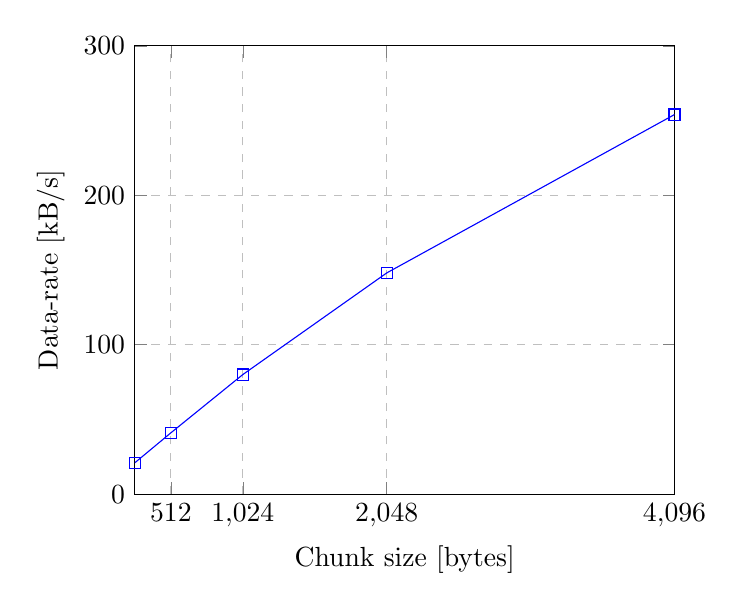
\begin{tikzpicture}
\begin{axis}[
    xlabel={Chunk size [bytes]},
    ylabel={Data-rate [kB/s]},
    xmin=256, xmax=4096,
    ymin=0, ymax=300,
    xtick={512,1024,2048,4096},
    xmajorgrids=true,
    ymajorgrids=true,
    grid style=dashed,
]
 
\addplot[
    color=blue,
    mark=square,
    ]
    coordinates {
    (256,21)(512,41)(1024,80)(2048,148)(4096,254)
    };
 
\end{axis}
\end{tikzpicture}
\caption{Write speeds for chunks of different sizes.}
\label{fig:write_speed}
\end{figure}

Given these results we have a memory/data-rate trade-off. Memory is limited on the micro-controller but we also want to maximise the amount of data that can be logged. In-field experimentation showed that under most circumstances write buffers of 2048 bytes are sufficient to achieve the data-rate necessary to log all sensor data. Nonetheless, we ended up using buffers of 4096 bytes to insure that no data would be lost.

\subsubsection{Comparison to Escher}

The most important objective in comparison to Escher was to improve the logging system. Already by introducing event-based logging more infrequent measurements can be logged less than more frequent measurements. As a result, higher data rates for more important data can be achieved by reducing the bandwidth used by less important measurements. More dramatically, the redesigned system logged on average 1355 data points per second at a data-rate of 29 kB/s, while the system on Escher achieved only a constant rate of 173,5 data points per second.

\begin{figure}[H]
\centering
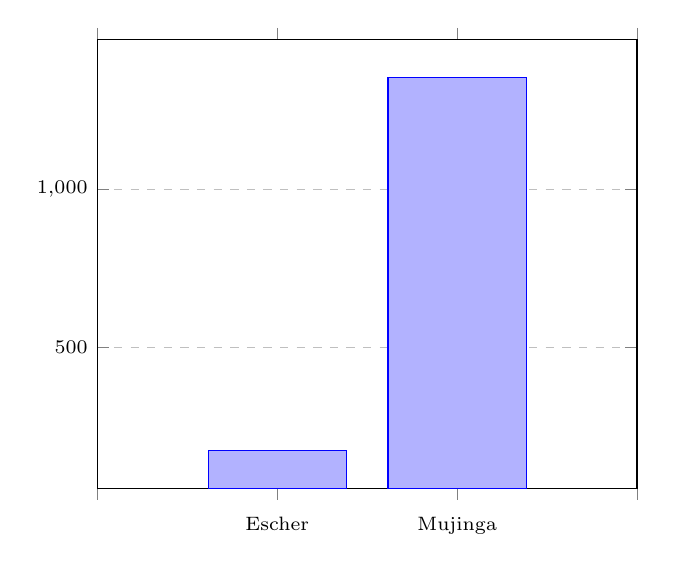
\begin{tikzpicture}
\begin{axis}[
        ybar,
        xtick={0,1,2,3},
        xticklabels={,Escher,Mujinga,},
        xticklabel style={yshift=-0.1cm},
        tick label style={font=\scriptsize},
        xmin=0,
        xmax=3,
        ymajorgrids=true,
        grid style=dashed,
        bar width=50pt
    ]

\addplot [
        blue,fill=blue!30
    ]
    coordinates {
        (1,173.5)(2,1355)
    };
\end{axis}
\end{tikzpicture}
\caption{Average number of logged data points per second.}
\label{fig:write_speed}
\end{figure}

\subsection{Networking}

Using an oscilloscope the SPI bus with the micro-controller and Ethernet controller can be monitored. Figures ~\ref{fig:net_send} and ~\ref{fig:net_recv} visualise the sequence of commands necessary for sending and receiving short 12 byte network packets. In order to send a packet, the micro-controller must first read the write pointer it should use from the Ethernet controller. Then it can write to the Ethernet controller's packet RAM at the read address. It must then update the write pointer so the Ethernet controller knows the length of the packet and finally confirm the packet using a send command. The sequence for receiving packets is analogous. Notice however, that the process is triggered by the interrupt signal from the Ethernet controller.

\begin{figure}[H]
    \centering \includegraphics[width=1.0\textwidth]{./figures/"SPI NET SEND".PNG}
    \caption{Command sequence for sending a network packet on SPI bus.}
    \label{fig:net_send}
\end{figure}

From Figure~\ref{fig:net_send} we can see that it takes only 39 microseconds to complete all commands necessary to send a network packet of this size at maximum clock rate supported by the SPI interface (12,5 MHz). The use of the DMA controller leads to uninterrupted transmission of each command on the bus. Although the demonstrated performance is more than fast enough for this application, the driver could still be optimised to reduce the time between commands. Some of the computation necessary for the next command is performed after the previous command is transmitted. Although this would increase memory usage, it could be performed while the previous command is still transmitting. On the other hand, for longer packets the time is dominated by the transmission subsequence labelled "write packet" in Figure~\ref{fig:net_send}.

The same optimisation could be applied to the reception of network packets but again Figure~\ref{fig:net_recv} shows that the full sequence only takes 47 microseconds, which is sufficient for this application. 

\begin{figure}[H]
    \centering \includegraphics[width=1.0\textwidth]{./figures/"SPI NET RECV".PNG}
    \caption{Command sequence for receiving a network packet on SPI bus.}
    \label{fig:net_recv}
\end{figure}

\section{In-Field Evaluation and Competition}

The control system was implemented specifically for the Hyperloop Pod Student Competition. It was extensively tested before the competition during functional tests and on a test 150m test track in Switzerland. During the competition the software was tested in several tests, most notably the functional test, navigation test and state diagram test.

\subsection{Pre-competition testing}

After checking the correct operation of all sensors and actuators in conjunction with the software, we checked that all emergency conditions and safety features worked correctly. Next, full pod operation was tested in a vacuum chamber. We were successfully able to spin up the motors in vacuum and all components operated nominally during the test. The pressurized battery compartments remained pressurized and the cells were therefore not damaged.

In addition to the vacuum chamber test, the team was able to use a 150m test track designed to match the specifications of the test tube at the competition. We completed several runs demonstrating correct operation of the navigational sensors, the navigation algorithm, the control of the inverters using both speed and torque commands, the control of the brake system and telemetry transmission and logging. Further test runs focused on applying maximal acceleration over short distances in order to fine-tune traction control.

\subsection{Competition}

%\todo{Pic: Mujinga at competition}

Throughout the competition week the pod was subjected to a wide range of tests. Three tests specifically target the control software developed in this thesis.

First, the functional test ensures that after power-on the pod is in a safe state and telemetry is received with nominal values. During this test the team also demonstrated correct operation of all safety-critical pod functions such as the brakes from software and using the control panel to command the pod.

Next, the navigation test verifies the navigational mechanisms built into the software work correctly and the level of fault tolerance is assessed. In order to show correct functionality of the navigational algorithm, all possible scenarios were simulated using fake optical markings while the pod remained stationary and the software responses were observed using the telemetry data visualised in the control panel.

Finally, the state diagram test consists of verifying the pod operates according to the state diagram (Figure~\ref{fig:state_diagram}). Essentially, this test checks that the global finite state machine is correctly implemented. To demonstrate this, all automatic transitions are tested by simulating all possible causes for the transition. For example, the transition \texttt{RUN} $\rightarrow$ \texttt{BRAKING} should occur after the pod has travelled a pre-defined distance. This can be simulated by passing fake optical markings in front of the laser contrast sensors.

With all these tests passed, the team had actually gained a decent lead compared to the other teams in the competition. The next test for the pod was the vacuum chamber test, where the full pod is placed in a large vacuum chamber. Although this test had been previously carried out successfully in Switzerland, the pod suffered a sever failure during this test preventing the team from advancing to the finals of the competition.

Shortly after enabling the high-voltage systems in vacuum, a loss of communications occurred. After re-pressurising the vacuum chamber it was immediately possible to see that the low-voltage electronics had been fatally damaged. Further investigation revealed, that the high-voltage batteries had been short circuited. Surprisingly, the low-voltage systems continued to log data for a full second after the failure. After analysing the data, the failure could be narrowed down to one of the inverters. A manufacturing fault caused arcing to occur between the two battery poles. The arcing damaged the inverter, portions of the low-voltage electronics, the low-voltage battery and both high-voltage batteries. Although we were able to repair all other components, the high-voltage battery cells were too severely damaged from the over current to be safely used any further.

\section{Conclusion}

In  conclusion, a control system was developed for a prototype Hyperloop pod and deployed at the Hyperloop Pod Competition hosted by SpaceX in Los Angeles, California. All major design goals could be met but some further optimization in some areas is possible. Although the team did not advance to the finals of the competition, the overall system was well designed and will provide a solid foundation for future Hyperloop projects.

%Summary of work

%What I did

%Quantitative data

%How it was used in the real world

%\section{Outlook}


%%%%%
%%%%% Start of additional parts.
%%%%%
\appendix

%%%%%%%%%%%%%%%%%%%%%%%%%%%%%%%%%%%%%%%%%%%%%%%%%%%%%%%%%%%%%%%%%%%%%%%
%%%%%%%%%%%%%%%%%%%%%%%%%%%%%%%%%%%%%%%%%%%%%%%%%%%%%%%%%%%%%%%%%%%%%%%
%%%%%                                                                 %
%%%%%     <file_name>.tex                                             %
%%%%%                                                                 %
%%%%% Author:      <author>                                           %
%%%%% Created:     <date>                                             %
%%%%% Description: <description>                                      %
%%%%%                                                                 %
%%%%%%%%%%%%%%%%%%%%%%%%%%%%%%%%%%%%%%%%%%%%%%%%%%%%%%%%%%%%%%%%%%%%%%%
%%%%%%%%%%%%%%%%%%%%%%%%%%%%%%%%%%%%%%%%%%%%%%%%%%%%%%%%%%%%%%%%%%%%%%%

%\chapter{Task Description}
%\includepdf[pages=-, turn=false, scale=0.9]{task/AufgabenstellungBachelorArbeitDINFKpdf.pdf}


\chapter{Declaration of Originality}\label{chap:originality}
Include the declaration of authorship with the \shell{\textbackslash
  includepdf} command (sign it and scan it). For more information
about plagiarism, please visit
\url{https://www.ethz.ch/students/en/studies/performance-assessments/plagiarism.html}

\begin{itemize}
\item \textbf{English version:}
  \url{https://www.ethz.ch/content/dam/ethz/main/education/rechtliches-abschluesse/leistungskontrollen/declaration-originality.pdf}
\item \textbf{German version:}
  \url{https://www.ethz.ch/content/dam/ethz/main/education/rechtliches-abschluesse/leistungskontrollen/plagiat-eigenstaendigkeitserklaerung.pdf}
\end{itemize}

% include the signed declaration of authorship!
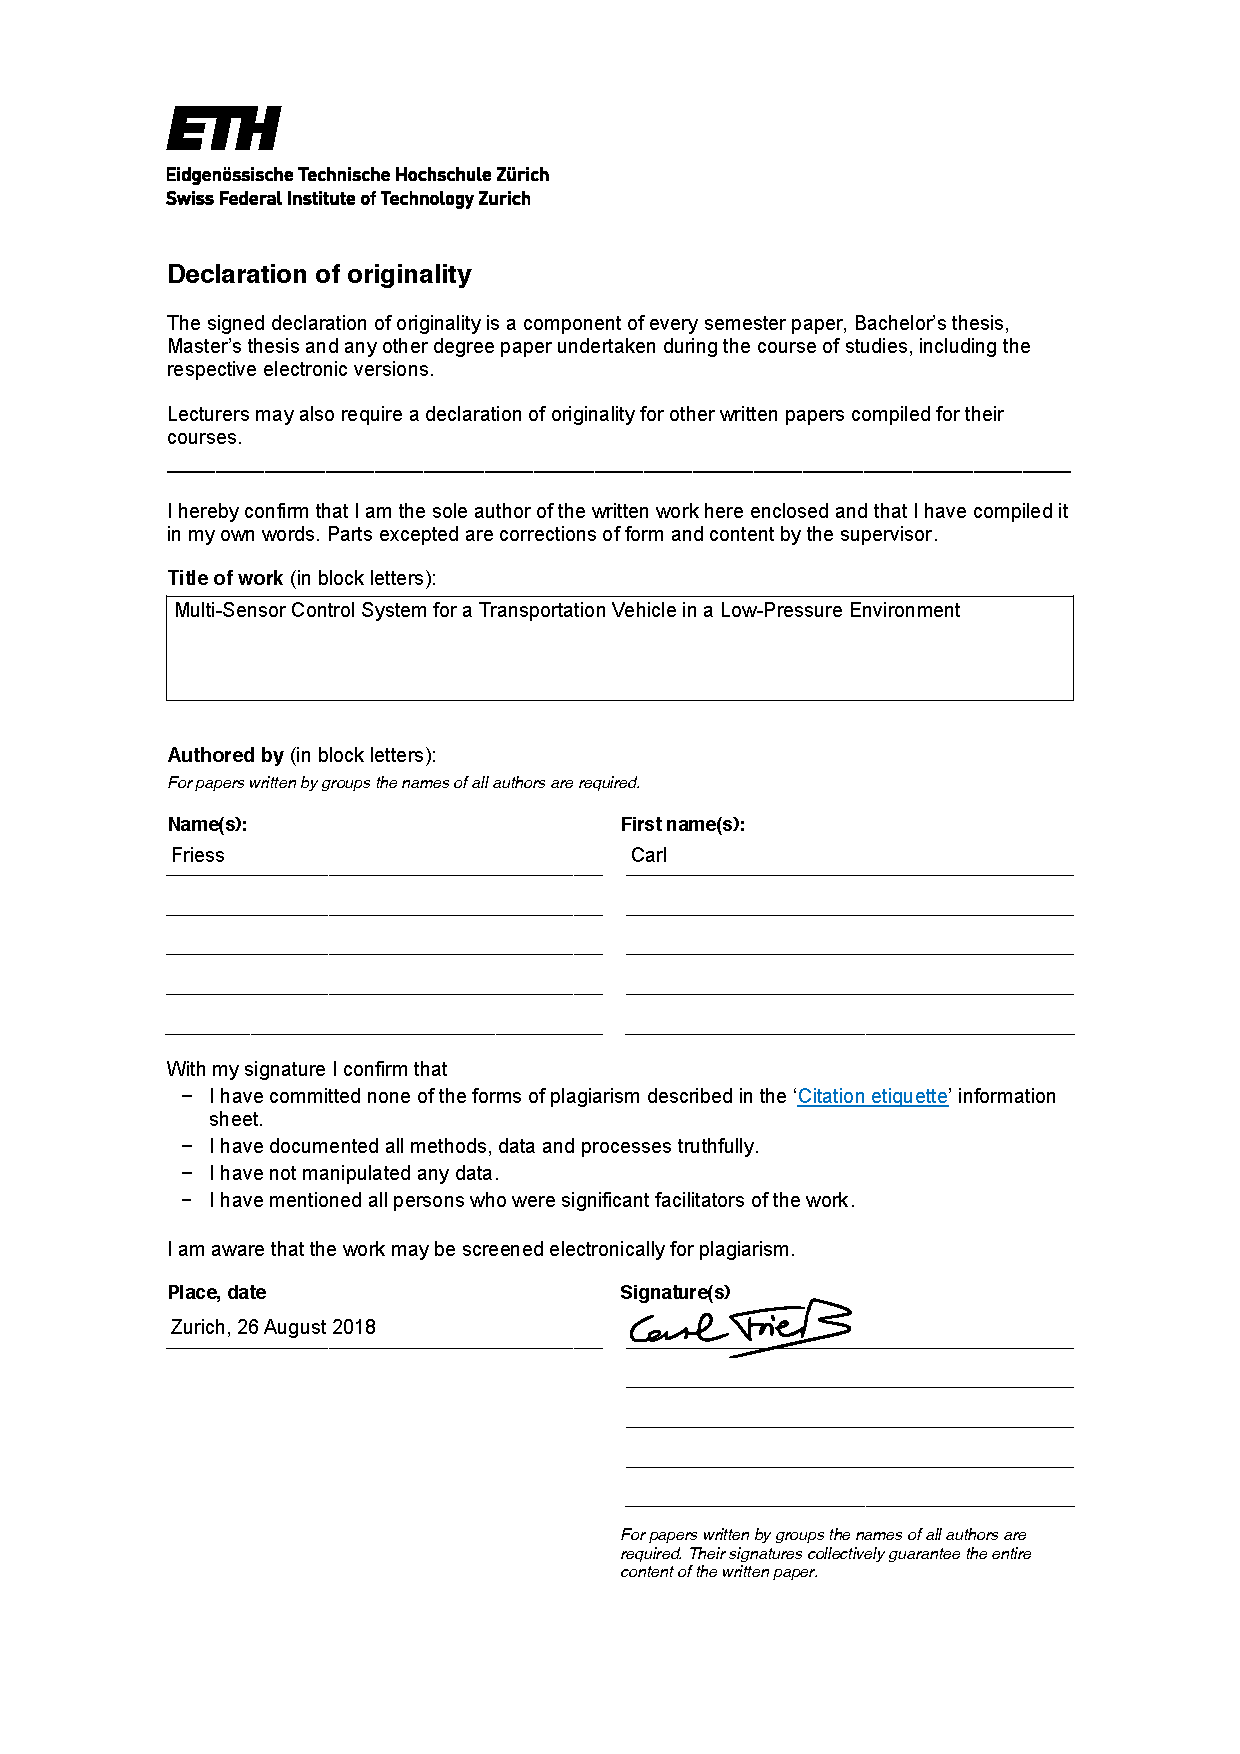
\includepdf[pages=-, turn=false, scale=0.9]{./figures/declaration_of_originality}


\backmatter

% Print the main glossary.
%\printglossary[type=main,title=Glossary]


% Print the bibliography.
\nocite*{} % Print non-cited references as well.
\bibliographystyle{IEEEtran}
\bibliography{IEEEabrv,./bib/main}


\end{document}
%%%%%%%%%%%%%%%%%%%%%%%%%%%%%%%%%%%%%%%%%%%%%%%%%%%%%%%%%%%%%%%%%%%%%%%
%%%%%                                                                 %
%%%%%     End of Document                                             %
%%%%%                                                                 %
%%%%%%%%%%%%%%%%%%%%%%%%%%%%%%%%%%%%%%%%%%%%%%%%%%%%%%%%%%%%%%%%%%%%%%%
